%%%%%%%%%%%%%%%%%%%%%%%%%%%%%%%%%%%%%%%%%
% Short Three-Column Newsletter
% LaTeX Template
% Version 1.0 (11/9/13)
%
% Original author:
% Frits Wenneker (http://www.howtotex.com) 
% With extensive modifications by:
% Vel (vel@latextemplates.com)
% 
% This template has been downloaded from:
% http://www.LaTeXTemplates.com
%
% License:
% CC BY-NC-SA 3.0 (http://creativecommons.org/licenses/by-nc-sa/3.0/)
%
%%%%%%%%%%%%%%%%%%%%%%%%%%%%%%%%%%%%%%%%%

%----------------------------------------------------------------------------------------
%	PACKAGES AND DOCUMENT CONFIGURATIONS
%----------------------------------------------------------------------------------------

\documentclass[10pt,a4paper]{article} % Paper type (a4paper, usletter or legal) and font size (10, 11 or 12)

\setlength\topmargin{-48pt} % Top margin
\setlength\headheight{0pt} % Header height
\setlength\textwidth{7.0in} % Text width
\setlength\textheight{9.5in} % Text height
\setlength\oddsidemargin{-30pt} % Left margin
\setlength\evensidemargin{-30pt} % Left margin (even pages) - only relevant with 'twoside' article option

\usepackage{charter} % Charter font for main content
\usepackage{siunitx}
\frenchspacing % Reduces space after periods to make text more compact for a three-column layout

\usepackage{graphicx} % Required for including images
\usepackage{amssymb,amsmath} % Math packages
\usepackage{multicol} % Required for the three-column layout of the document
\usepackage{url} % Clickable links
\usepackage{enumitem} % Reduces the amount of space within and between lists with [noitemsep,nolistsep]
\usepackage{marvosym} % Required for the use of symbols
\usepackage{wrapfig} % Allows wrapping text around figures
\usepackage[T1]{fontenc} % Use 8-bit encoding that has 256 glyphs
\usepackage{datetime} % Required for defining a custom date style
\newdateformat{mydate}{\monthname[\THEMONTH] \THEYEAR} % Set a custom date format
\usepackage[pdfpagemode=FullScreen, colorlinks=false]{hyperref} % Link colors and PDF behavior in Acrobat
\usepackage{fancyhdr} % Required to define custom headers/footers
\pagestyle{fancy} % Enables the custom headers/footers for all pages following this

%-----------------------------------------------------------
% Header and footer
\lfoot{\footnotesize % Left footer containing newsletter contact information
	Greek islands, a paradise on earth\\
	\Mundus\ \href{https://github.com/stefanos1316/my_blog/index.com}{my\_blog/index.com} \quad
	%\Telefon\ Not available yet \quad
	\Letter\ \href{mailto:sgeorgiou@aueb.gr}{sgeorgiou@aueb.gr}
}


\cfoot{} % Empty center footer

\rfoot{\footnotesize ~\\ Page \thepage} % Right footer - page counter

\renewcommand{\headrulewidth}{0.0pt} % No horizontal rule for the header
\renewcommand{\footrulewidth}{0.4pt} % Horizontal rule separating the footer from the document
%-----------------------------------------------------------

%-----------------------------------------------------------
% Define separators
\newcommand{\HorRule}[1]{\noindent\rule{\linewidth}{#1}} % Creates a horizontal rule
\newcommand{\SepRule}{\noindent	% Creates a shorter separator rule
\begin{center}
\rule{250pt}{1pt} % Page width and rule width
\end{center}
}
%-----------------------------------------------------------

%-----------------------------------------------------------
% Define title and article styles
\newcommand{\NewsletterName}[1]{ % Newsletter title
\begin{center}
\Huge \usefont{T1}{fvs}{b}{n} % Use the Bera Sans Bold font
#1
\end{center}	
\par \normalsize \normalfont}

\newcommand{\JournalIssue}[1]{ % Date and issue number at the top of the newsletter
\hfill \textsc{18th of May 2018, No #1} % Right-aligned date and issue number
\par \normalsize \normalfont}

\newcommand{\NewsItem}[1]{ % News item title
\usefont{T1}{fvs}{n}{n} % Use the Bera Sans Normal font
\vspace{24pt}\large #1\vspace{3pt} % Print the title with space around it in a larger font size
\par \normalsize \normalfont}

\newcommand{\NewsAuthor}[1]{ % Author name under the item title
\hfill by \textsc{#1} \vspace{20pt} % Right-aligned author name in small caps with space after it
\par \normalfont}		

%----------------------------------------------------------------------------------------
%	TITLE
%----------------------------------------------------------------------------------------

\begin{document}

\JournalIssue{1} % Issue number

\NewsletterName{Visiting the paradise islands} % Newsletter title

\noindent\HorRule{3pt} \\[-0.75\baselineskip] % Thick horizontal rule
\HorRule{1pt} % Thin horizontal rule

%----------------------------------------------------------------------------------------
%	MAIN NEWS ITEM
%----------------------------------------------------------------------------------------

\vspace{0.5cm}
\SepRule
\vspace{-0.5cm}

\begin{center}
\begin{minipage}[h]{0.84\linewidth}
\begin{wrapfigure}{l}{0.44\textwidth}
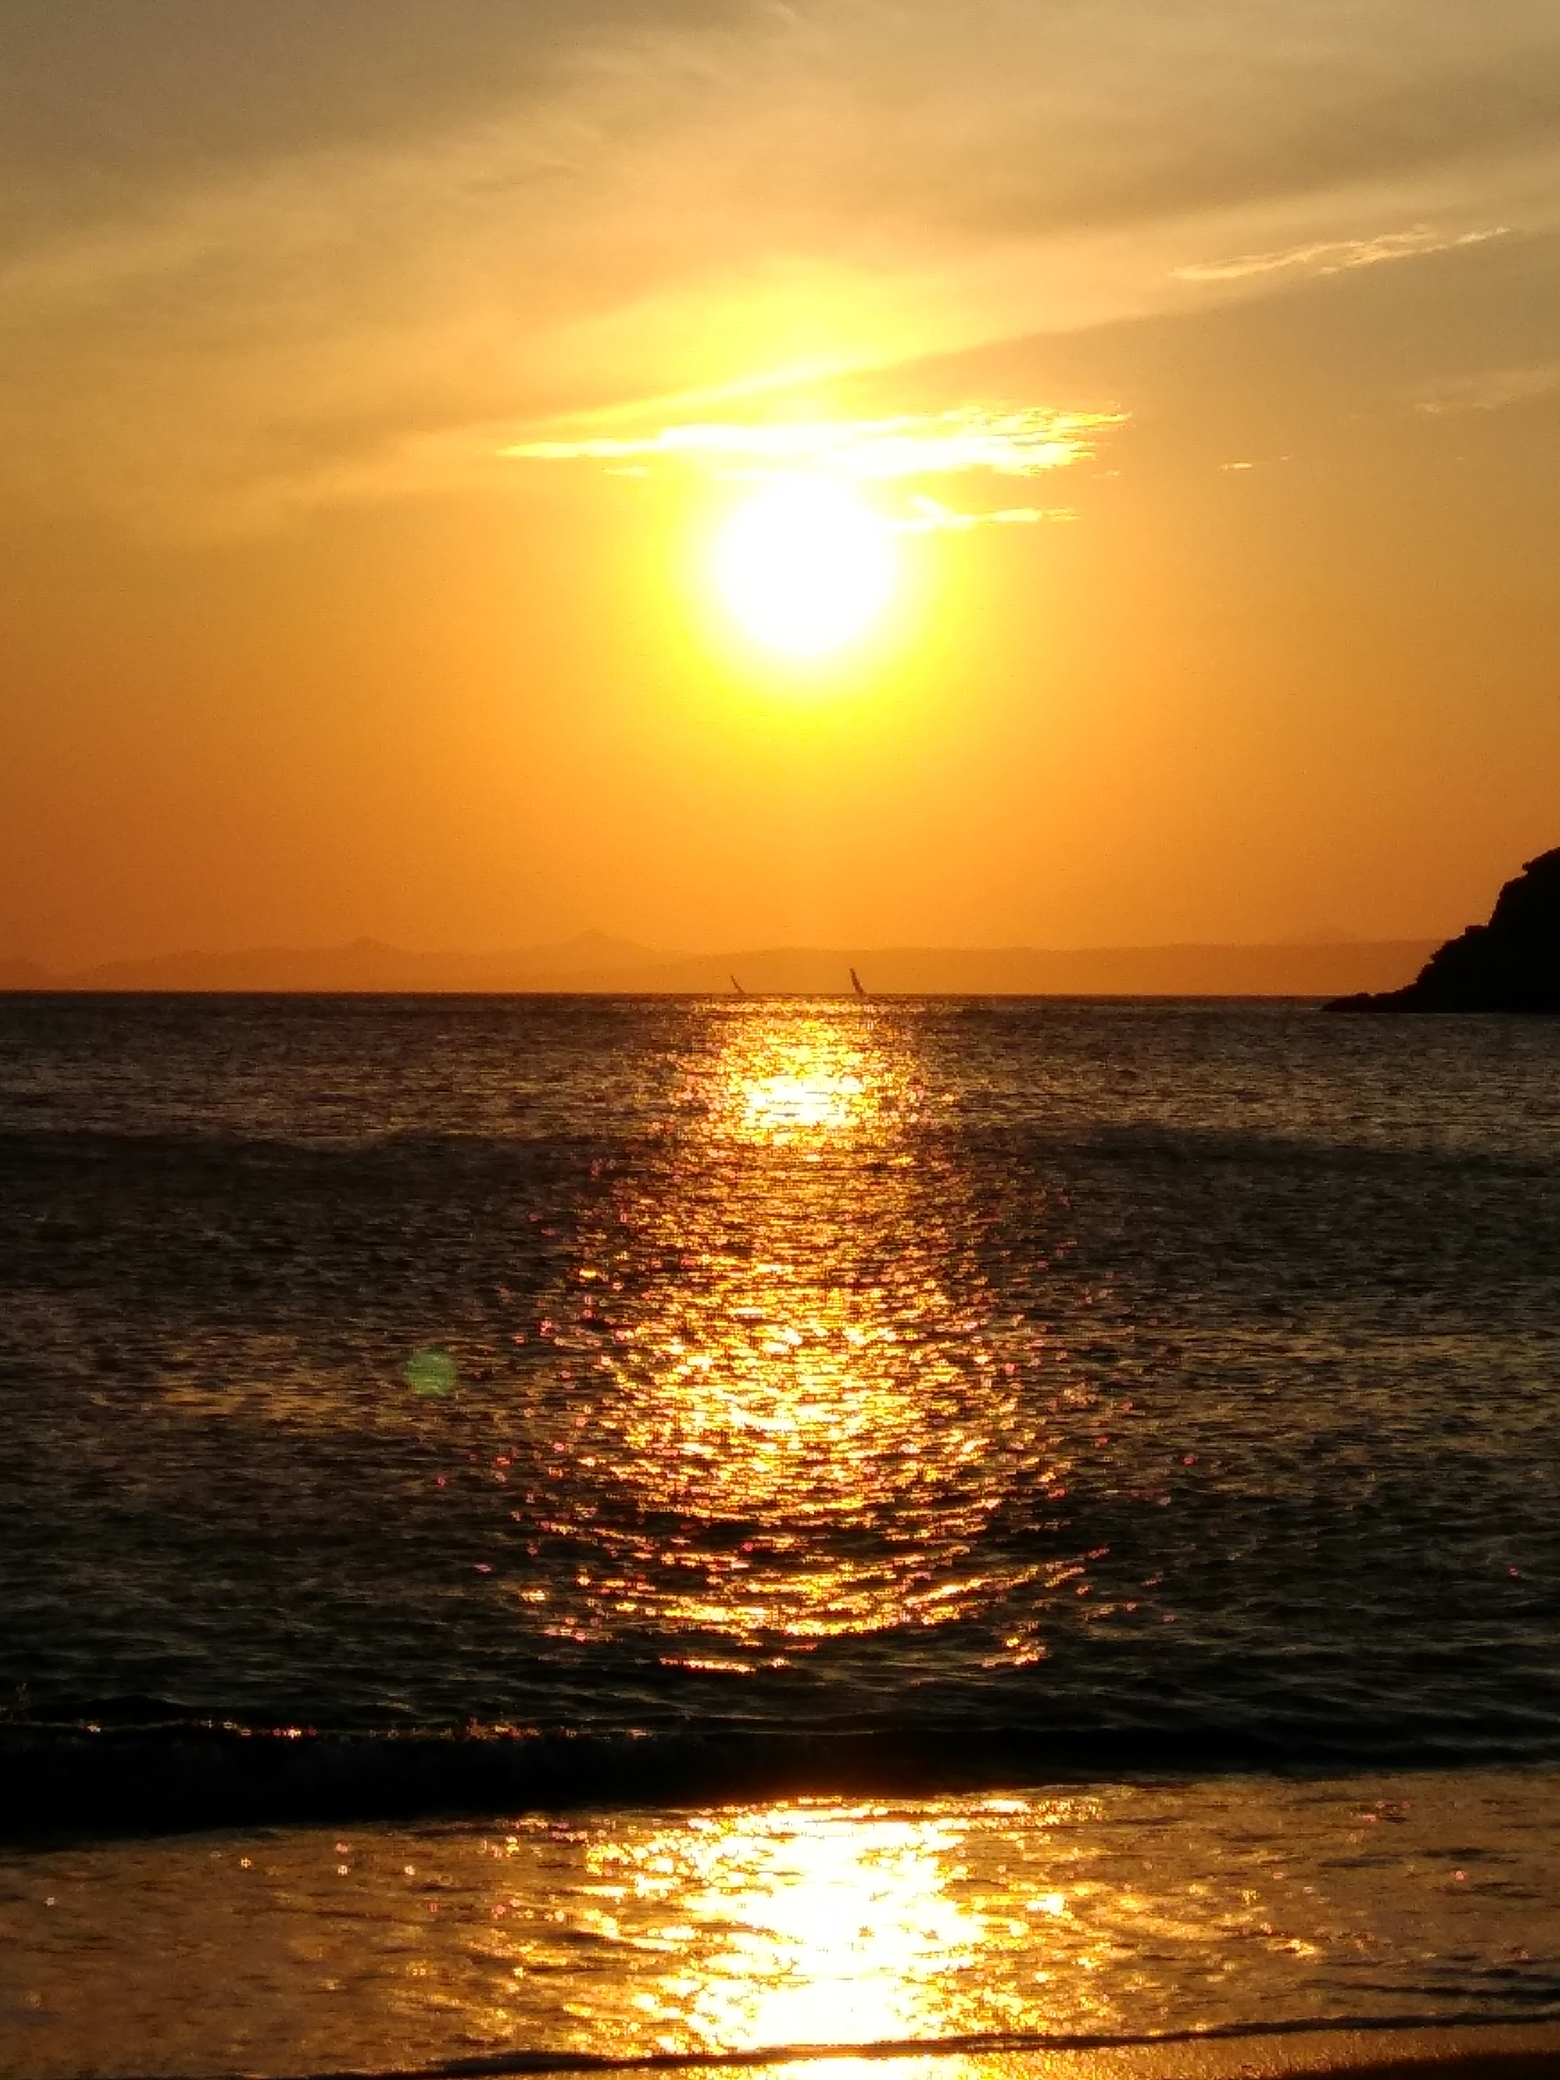
\includegraphics[width=0.4 \textwidth]{media/front_picture.jpg}
\\
\end{wrapfigure}
	
\NewsItem{Author's thoughts} % Main next item title
\vspace{3pt} % Some extra whitespace since there is no author as for the news in the body of the newsletter
\textit{
Greece, the country of democracy, the birthplace of great philosophers and scientists, 
the country of culture and art, but also a country that does not lack environmental 
beauty. 
This charm of Greece's environmental beauty lies in the vast number of islands which offer 
simplicity, relaxation, and endless moments of happiness. 
A pleasant feeling covers me upon landing on an island; the adventurous feeling 
is immediately born and a desire of discovering it feels me in every time. 
Before start pursuing my Doctorate degree, in Athens, I have never visited any 
Greek island before. 
However, after starting visiting them, my jaws dropped every time. 
A feeling of enthusiasm covers my mind of each islands unique character, 
their different way of living, and the openness of their locals.
Many times, I catch my self thinking the same thing, ``when I become pensioner I am 
going to by a small house in a Greek island and living a chill, quiet, and easy 
going live...''
}
\par\hfill --- Stefanos Georgiou
\end{minipage}
\end{center}

\vspace{0.5cm}
\SepRule % Small horizontal rule after the main news item
\vspace{0.5cm}

%\setlength{\columnsep}{16pt} % Uncomment to manually change the white space between columns
\begin{multicols}{3} % Begin the three-column layout

%----------------------------------------------------------------------------------------
%	OTHER NEWS
%----------------------------------------------------------------------------------------

\NewsItem{A visit in Haven}
\NewsAuthor{Stefanos Georgiou}
In 2010, Greece was officially announced as a country of economic crisis, 
a fact that goes on over eight years, nowadays. 
However, Greece is never on crisis on the unimaginable beauty and charm 
of its environment and more specifically its islands. 
The combination of sunny weather, almost all year along,
with the substantial and tasty portions of food, the great hospitality of its people, and the 
intense nightlife are the reasons making many tourists daydreaming when they talk 
about Greece all over the world.

According to Wikipedia, Greece has around 1,200 to 1,600 islands where 227 
are inhabited. 
It also offers beaches with various sandy colours such as brown, white, golden, 
pink, and volcanic black. 
Alongside, it is a country with the most blue flagged beaches in Europe that 
indicates the clean waters. 
Tourists can enjoy their stay in islands through hotels, Airbnb apartments, 
or even camping sites which various of them do exist. 
However, my suggestion is not to stay for a long time at hotel resorts, but, instead 
travel to different villages, talk with locals, go the places that also locals 
go to learn from this culture.

Through my stay in Greece,
I was fortunate to visit at least ten different islands from various seas.
Greece's islands can be found both in Aegean and Ionian seas. 
The distinguishing aspects of Aegean islands is the dry climate and environment,
but, warm seas. 
On the contrast, Ionian islands are less dry with a rich environment
and many trees, but, with much colder waters, in general. 
The Greek islands are group in six clusters: the \textit{Argo-Saronic},
\textit{Cyclades}, \textit{North Aegean}, \textit{Dodecanese},
\textit{Sporades}, \textit{Ionia} islands also know as \textit{Eptanisa}, 
and \textit{Crete} that is a single large island.
I have toured islands in both seas but primarily from the Aegean sea. 
Therefore most of the discussion is going to be for the Aegean islands. 

My aim with this article is to expose the hidden magic of the islands
through some of my adventures, feelings, historical events,
and thoughts to encourage people that paradise is not far away,
it is much closer than most of them think. 
  
\NewsItem{Aigina, my first island}
By the end of April 2016, when the temperature usually is much higher than \ang{30}, 
a friend of mine, that we used to server in army for our mandatory duty, gave me 
an unexpected call. 
He was visiting Athens with his girlfriend for few days and he wanted to travel to 
Aigina and to catch up with me.
A relatively big islands that is located at Sarronic bay and less than an hour 
distance away from Pireaus port by boat and famous mostly for the Aigina's peanuts; 
which is actually...a kind of pistachio. 


%12345678901234567890123456789012345678901234567890123456789012345678901234567890
Until that time, I have never been before to any island nor on a boat and since 
I am always up for trying new a different things I took the call. 
In general, in low season, there is no need to pre-book boat tickets since not 
many people are visiting the islands. 
After we bought our tickets, we entered the boat and took a place outside where 
to have better view and stair the seagulls. 
The seagulls were flying most of the time next to the boat to fish. 
Many people were trying to feed them in order to take pictures with them. 
It is necessary to be careful since the seagulls can bite also your hand while 
trying to get the food out of it. 
Therefore, we enjoy the view until we reached our destination, the port of Aigina. 


\begin{center}
	\includegraphics[width=0.32\textwidth]{media/aigina_2.jpg}
	\par\textit{Aigina's port and clean waters}
\end{center}


%12345678901234567890123456789012345678901234567890123456789012345678901234567890
The port of Aigina, where we disembarked, is located in the main city. 
Each island of Greece has its own main city and in most case a port can also be 
found there. 
In the old times, for some islands, the locals were building their main cities 
on mountains away from the port. 
This was done since to avoid quick attacks from pirates. 
However, it was not the case for Aigina. 


\begin{center}
	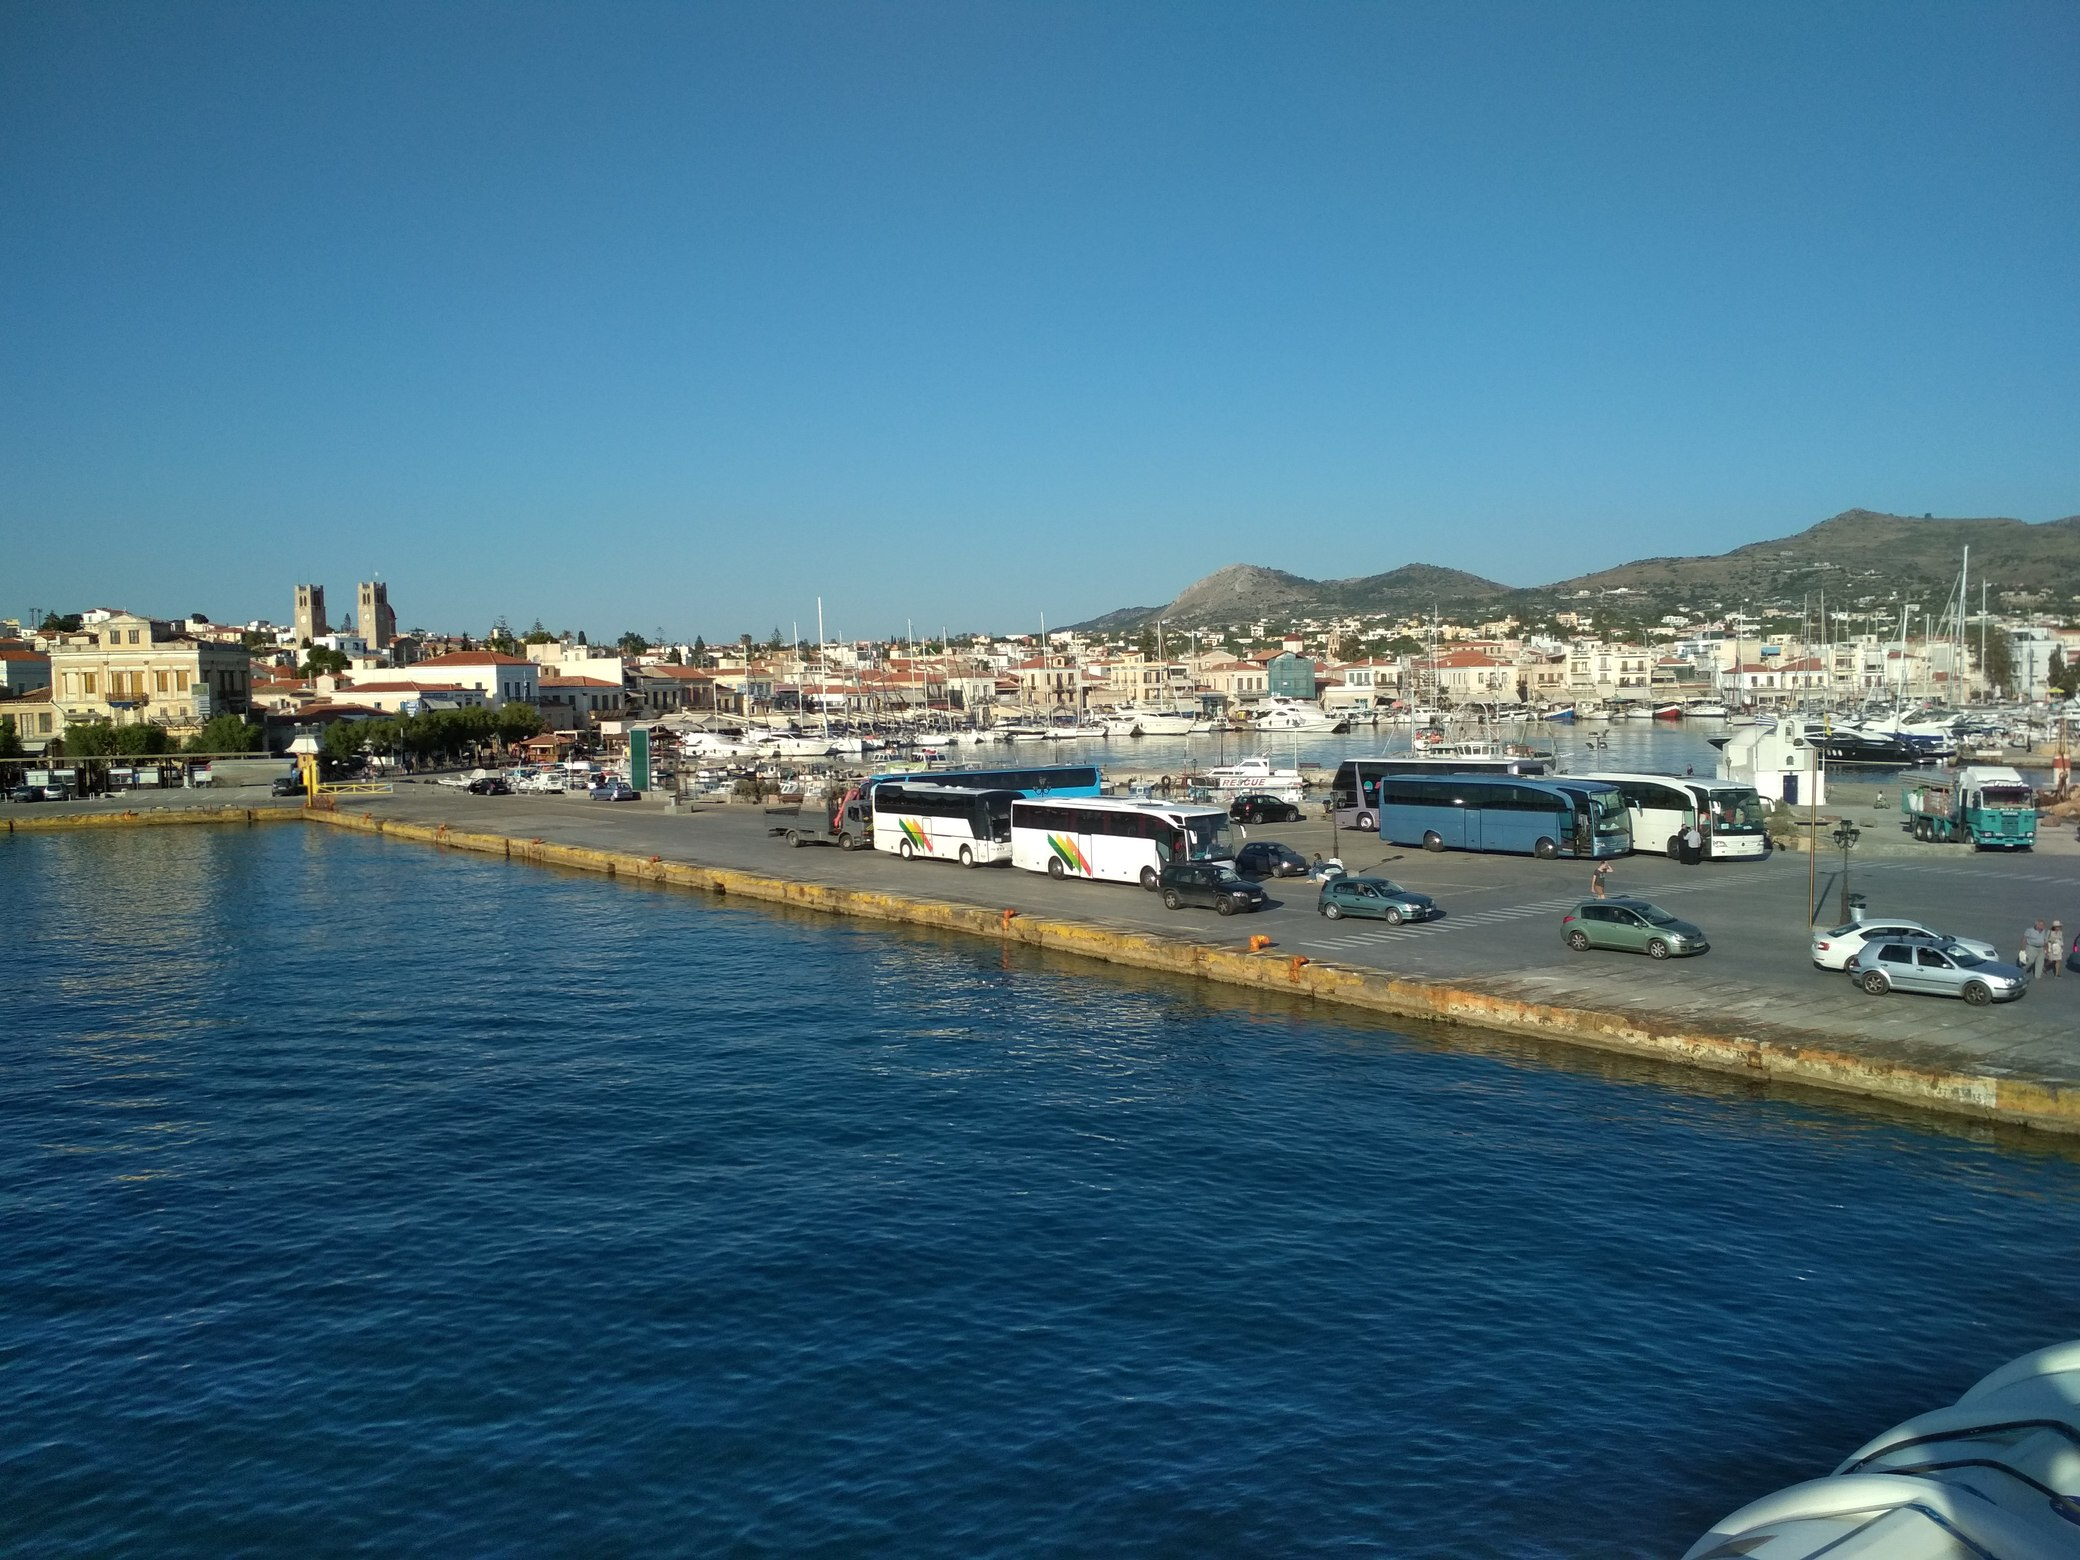
\includegraphics[width=0.32\textwidth]{media/aigina_3.jpg}
	\par\textit{Aigina's main city}
\end{center}


%12345678901234567890123456789012345678901234567890123456789012345678901234567890
Once we disembarked, we took a ride towards Marathonas beach since it is found 
outside of the city and the bus schedules are not in favour of the public. 
However, on my second tour to Aigina I was more prepared and I rented a bike which 
was much fun and a cheaper solution.
The organised beaches in Greece offer umbrellas, beach beds, and bars from where 
you can enjoy ice-cold coffees such as frappe, cold beers, and different snacks. 
Even tho it was May and the outside temperature more that \ang{35} the water was 
quite cold for my Cypriot standards. 
Nevertheless, it was also refreshing and my first bath, so I tried to enjoy it 
as much as I could without showing that it was cold. 


%12345678901234567890123456789012345678901234567890123456789012345678901234567890
After our cold experience on Marathonas beach, we made our way back to the city 
where we enjoyed some local food and Aigina's peanuts. 
Also, we took our time to explore the city centre that provides different types of 
restaurants, mainly we Greek cuisine,  and small narrow roads where decorated with 
many bougainvillea, white house, and very clean streets. 
Just walking in those streets of Aigina you can get the feeling that some things 
in that island remained unaffected by the past of time. 
But still, the beauty and their simplicity can rest the humans soul. 
After our walk we took the boat to return to the noisy Athens once again.


%----------------------------------------------------------------------------------------
\NewsItem{Salamina}

%12345678901234567890123456789012345678901234567890123456789012345678901234567890
A place where one of the biggest naval battle between the Greece and the Persian 
army took place. 
On that time, Greece was separated in different kingdoms. 
Therefore, they united their forces to take down their common enemy. 
Also, there is a large naval base at Salamina that is hosting multiple types of 
warships.


%12345678901234567890123456789012345678901234567890123456789012345678901234567890
By the begging of May 2016, one of our lab's PhD fellow, Maria Kechagia, invited 
the whole lab in her hometown, which is in Salamina for a day trip. 
Salamina, is an island that is almost 15 minutes away by ferry boat. 
Therefore, we took the opportunity and we loaded two cars in the ferry to make our 
way easier in Salamina. 
The different between the ferry and the normal boat is that the ferry is much 
smaller and slower. 
That means strong waves and long distances are troublesome.


\begin{center}
	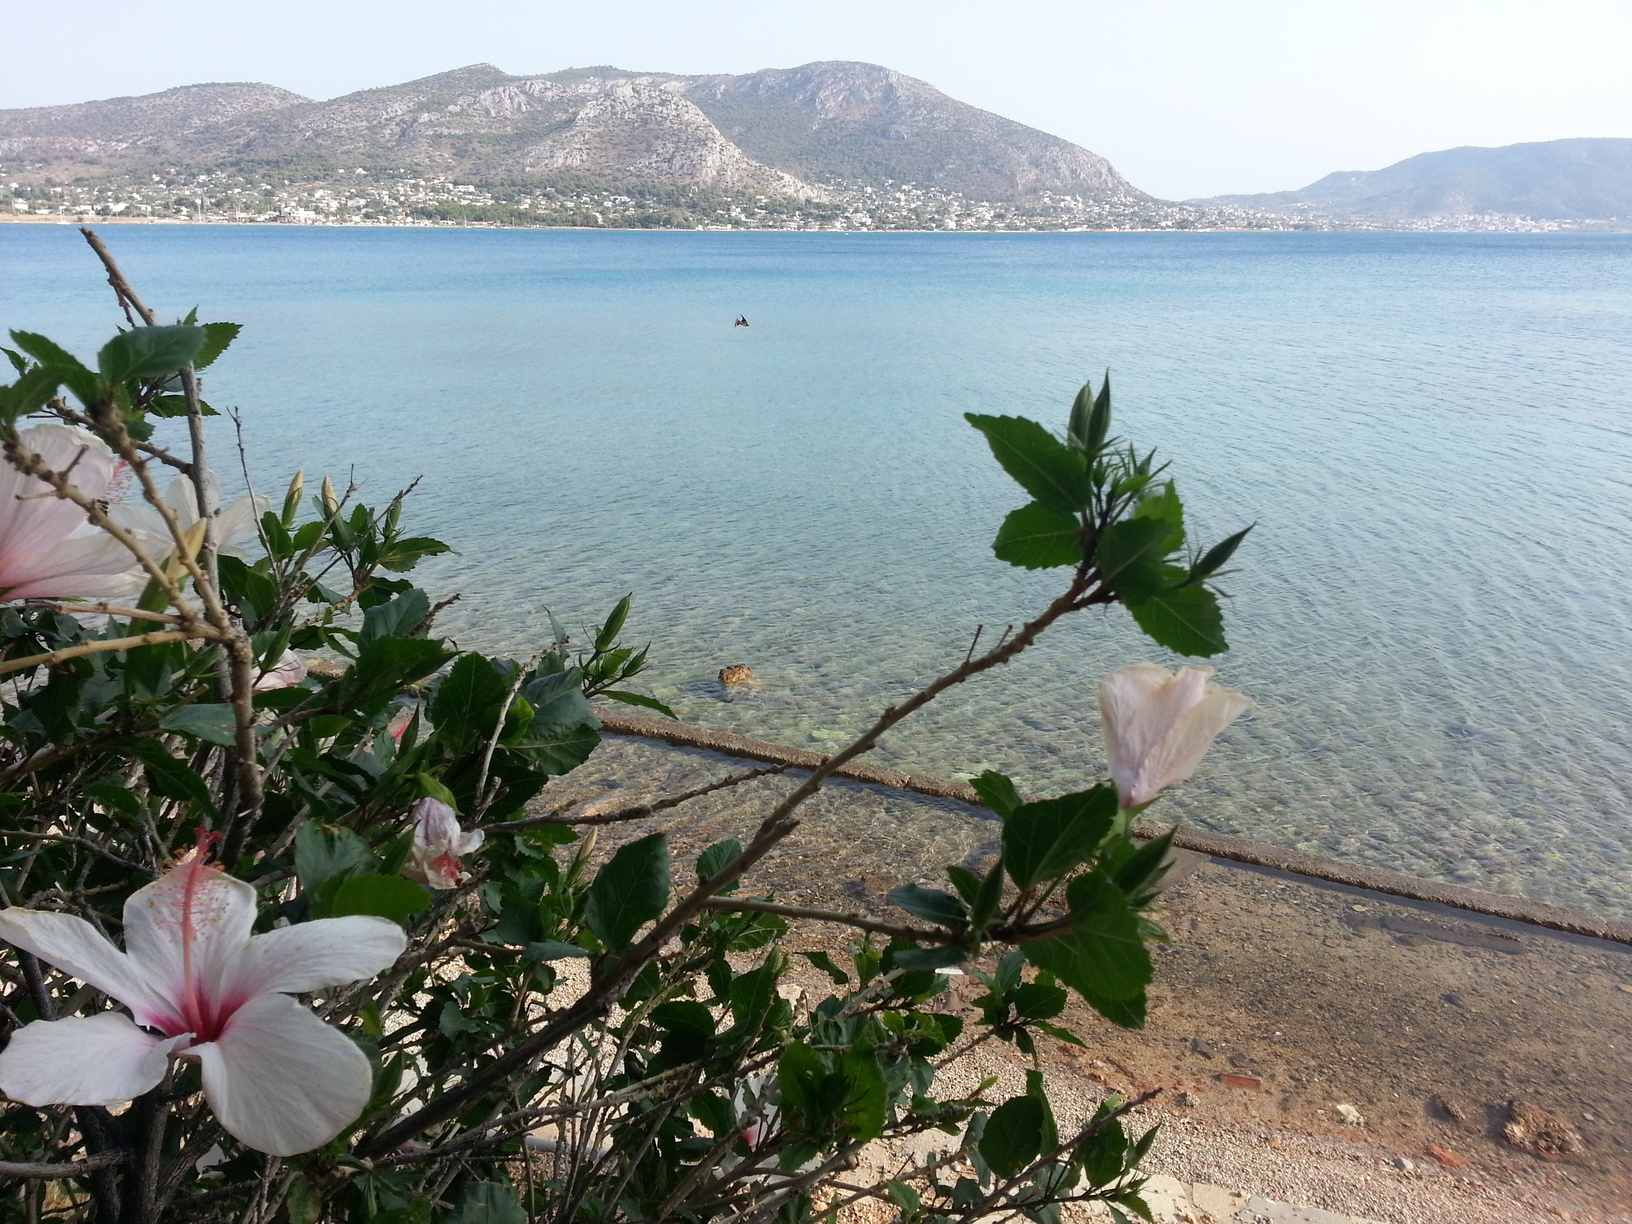
\includegraphics[width=0.32\textwidth]{media/salamina_1.jpg}
	\par\textit{The island of Salamina}
\end{center}


%12345678901234567890123456789012345678901234567890123456789012345678901234567890
Our first stop in Salamina was at Maria's home where her parents were expecting us. 
Her mother, few months ago had to go through a surgery and blood was required for 
that. 
Upon request, I immediately went for blood donation, a fact that her mother remembers 
till today and every time we meet she is bringing me cookies and other kind of sweets. 
In our company, we also had a PhD student from India who came with his wife and 
four years old kid. 
Greek parents are going crazy when they see kids and they try to cheer them with 
every kind of sweet of toys they have, no matter from which country they are. 
However, they did not only treat the kid well but us also. 
Once we sit outside in their garden that was full of trees, plants and flowers, 
Maria's mother brought us coffee, cookies, and home made ice-cream. 
Afterwards, they also suggested us beaches to visit and places to eat lunch.


\begin{center}
	\includegraphics[width=0.32\textwidth]{media/salamina_2.jpg}
	\par\textit{Beach in Salamina}
\end{center}


%12345678901234567890123456789012345678901234567890123456789012345678901234567890
After the beach we went to have lunch at a local restaurant where we order ``kotsi''. 
This food is part of the pork's leg, cooked in an oven with sauce and different 
species. 
Literally the meat was going off the bone by simple touching it. 
It was one of the most amazing ``kotsi'' we ever had. 
Even after two years, our PhD fellow Antonis Gkortzis is still mentioning that food.     


%----------------------------------------------------------------------------------------
\NewsItem{Vacations in Milos}

%12345678901234567890123456789012345678901234567890123456789012345678901234567890
Summer in Athens is almost unbearable and an escape plan is go to a Greek island. 
Ana, a beautiful blond Slovenian girl with charming blue eyes 
and a crystal smile, came to visit me in order to go at Milos island. 
Milos is an island in Cyclades before Santorini, however, much more 
cheaper, with less tourists, and beautify sandy beaches. 
In addition, most of the Cyclades islands share the common characteristics as 
white houses, flat roofs, blue doors and window labels, in most of cases. 
Therefore, in mid of July 2016 we travelled there by boat that took us more than four hours to reach 
our destination. 


%12345678901234567890123456789012345678901234567890123456789012345678901234567890
Milos has many beaches that are inaccessible by cars or foot and to visit them 
a sailing boat is required. 
To this end, we booked a whole day sailing tour with Ana to explore and enjoy 
the hidden places of Milos. 
Again, for me, it was my first time travelling by sailing boat, an  experience 
which came to be fascinating and enjoyable since I love snorkelling and sailing 
boats offer this opportunity in a large scale. 
Also, we went close to an island called Poliaignos. 
A rocky island next to Milos that is mostly inhabited but goats and the 
shepherds that are watching over them.
Poliaigos had the most clear blue water I have ever seen in my life. 
Even tho the water's depth was more than 15 meters the bottom was quite 
visible, but, also cold.

\begin{center}
	\includegraphics[width=0.32\textwidth]{media/milos_poliaigos.jpg}
	\par\textit{The crystal blue waters of Poliaigos}
\end{center}
  

%12345678901234567890123456789012345678901234567890123456789012345678901234567890
From the sailing boat, we also saw some of the traditional fisher men houses.  
The fisher men were colouring their houses doors with different colours 
to recognise them during night. 
This was done to avoid anchoring their boat outside the wrong parking spot.

\begin{center}
	\includegraphics[width=0.32\textwidth]{media/milos_houses.jpg}
	\par\textit{Fisher men houses in Milos}
\end{center}


%1234567890123456789012345678901234567890123456789012345678901234567890123456789
During the night, our sailing trip reached its end. 
Overalls, the trip was tiresome since the wavy sea forced us to try keep our 
balance, in the boat, most of the time and in combination with the strong sun 
we get exhausted. 
However, it was a great new adventurous experience for me and one that 
I definitely repeat. 
In addition, we have visited coast lines that we could never see by car and it 
made it worth our time and the energy we spend on the trip. 


%1234567890123456789012345678901234567890123456789012345678901234567890123456789
A rather daring act from us was to use the local buses for transportation which 
end up being a cumbersome and time costly action. 
Many times, we ended up at completely wrong places and far away from our 
destination. 
However, every time locals where stopping to give us drive and to talk to us. 
In addition, they were really interested in our own stories too and many times 
they were suggesting us places for meals with the best value for many deals. 
Also, an old guy took us with his car at one of the most beautiful beaches of 
Milos, the Firiplaka beach. 


\begin{center}
	\includegraphics[width=0.32\textwidth]{media/milos_beach.jpg}
	\par\textit{Me at Firiplaka beach}
\end{center}


%1234567890123456789012345678901234567890123456789012345678901234567890123456789
Firiplaka is an magnificent golden sandy beach with blue and clear waters 
as depicted in the above picture. 
The specific beach is partially organised while the biggest part of it is not. 
It offers a small number of umbrellas and sea beds free of use with the policy 
of first come first serve. 
Also, it has a small kiosk that offers a number of refreshments, snacks, tasty 
and big bowls with Greek yoghurt with various seasonal fruits, walnuts, and honey 
for very reasonable prices. 


%1234567890123456789012345678901234567890123456789012345678901234567890123456789
A different type of beach is the Sarakiniko. 
Sarakiniko means piratear and it is a white rocky bay as illustrated in the 
picture below. 
Its schema offers warm and ease waters to its swimmers with a small beach surrounded 
by many fig trees. 
As it is among the famous places of Milos and most of the time is quite crowded. 
However, it offers many spots and people can also lay on the rocky parts too.


\begin{center}
	\includegraphics[width=0.32\textwidth]{media/milos_beach_2.jpg}
	\par\textit{The Sarakiniko beach}
\end{center} 


%1234567890123456789012345678901234567890123456789012345678901234567890123456789
After we left from the beach, we made our way towards Plaka of Milos to enjoy the 
sun set. 
Plaka is small city located on a hill in the centre of the island. 
It also offers a number of restaurants, bars, and cafeterias from where you can 
see the sun set. 
For dinner, we had a delicious shrimps with cheese form Milos and grilled vegetables 
at a local restaurant while we enjoyed cold Mythos beer. 
Moreover, we didn't waste our chance to enjoy the sun set while listening to Hans 
Zimmer's songs such as ``The last of Mochicans'', ``Braveheart'', and so on, a 
tradition that I acquired from my PhD fellow Antonis Gkortzis and I still follow.


\begin{center}
	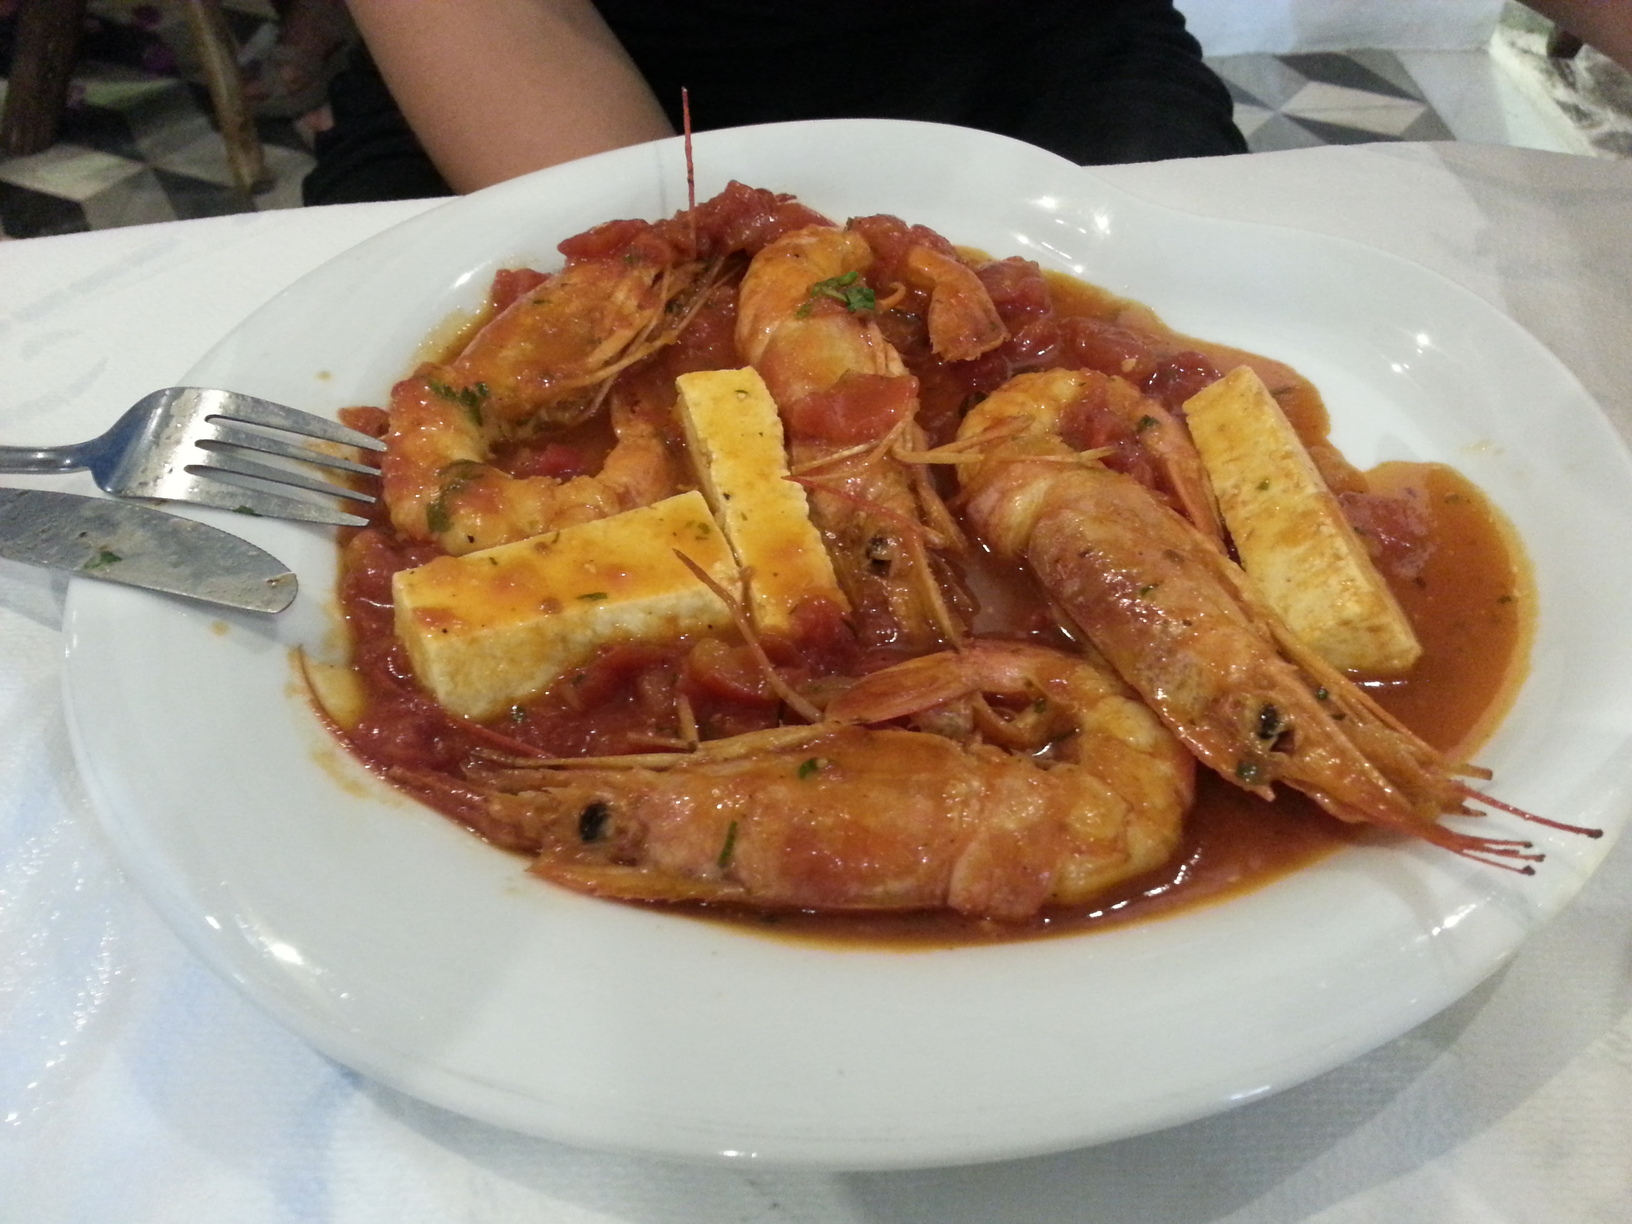
\includegraphics[width=0.32\textwidth]{media/milos_food.jpg}
	\par\textit{Shrimps with cheese from Milos}
\end{center}


%----------------------------------------------------------------------------------------
\NewsItem{My dream is to fly}

%1234567890123456789012345678901234567890123456789012345678901234567890123456789
After returning from Milos I received news that a dear friend of mine from Serbia, 
Vojkan Stoitsik (a cool University assistant professor at Greek literature), 
was going for vacations at Lefkada island. 
Lefkada is big island found at the Ionian sea with rich environmental beauty, a lot 
of trees, and cold waters.
In order to visit my friend for two days, since I took most of my days off, I 
booked a bus tickets towards Lefkada. 
Well, next time I should be more careful with the time tables since it was eight hours 
of bus driving which depleted my energy until I reached my destination. 
Needless to say, I have spend around 16 hours just for driving while I stayed at 
Lefkada almost a day. 


%1234567890123456789012345678901234567890123456789012345678901234567890123456789
The island of Lefkada is connected with the main part of Greece through a bridge 
since it is very close, thus no boat is required to reach it. 
It also has a very beautiful and traditional city centre that offers many 
restaurants, cafeterias, and bar. 
In addition, next to port many bars and night clubs can be found with loud 
music and fancy lights. 

\begin{center}
	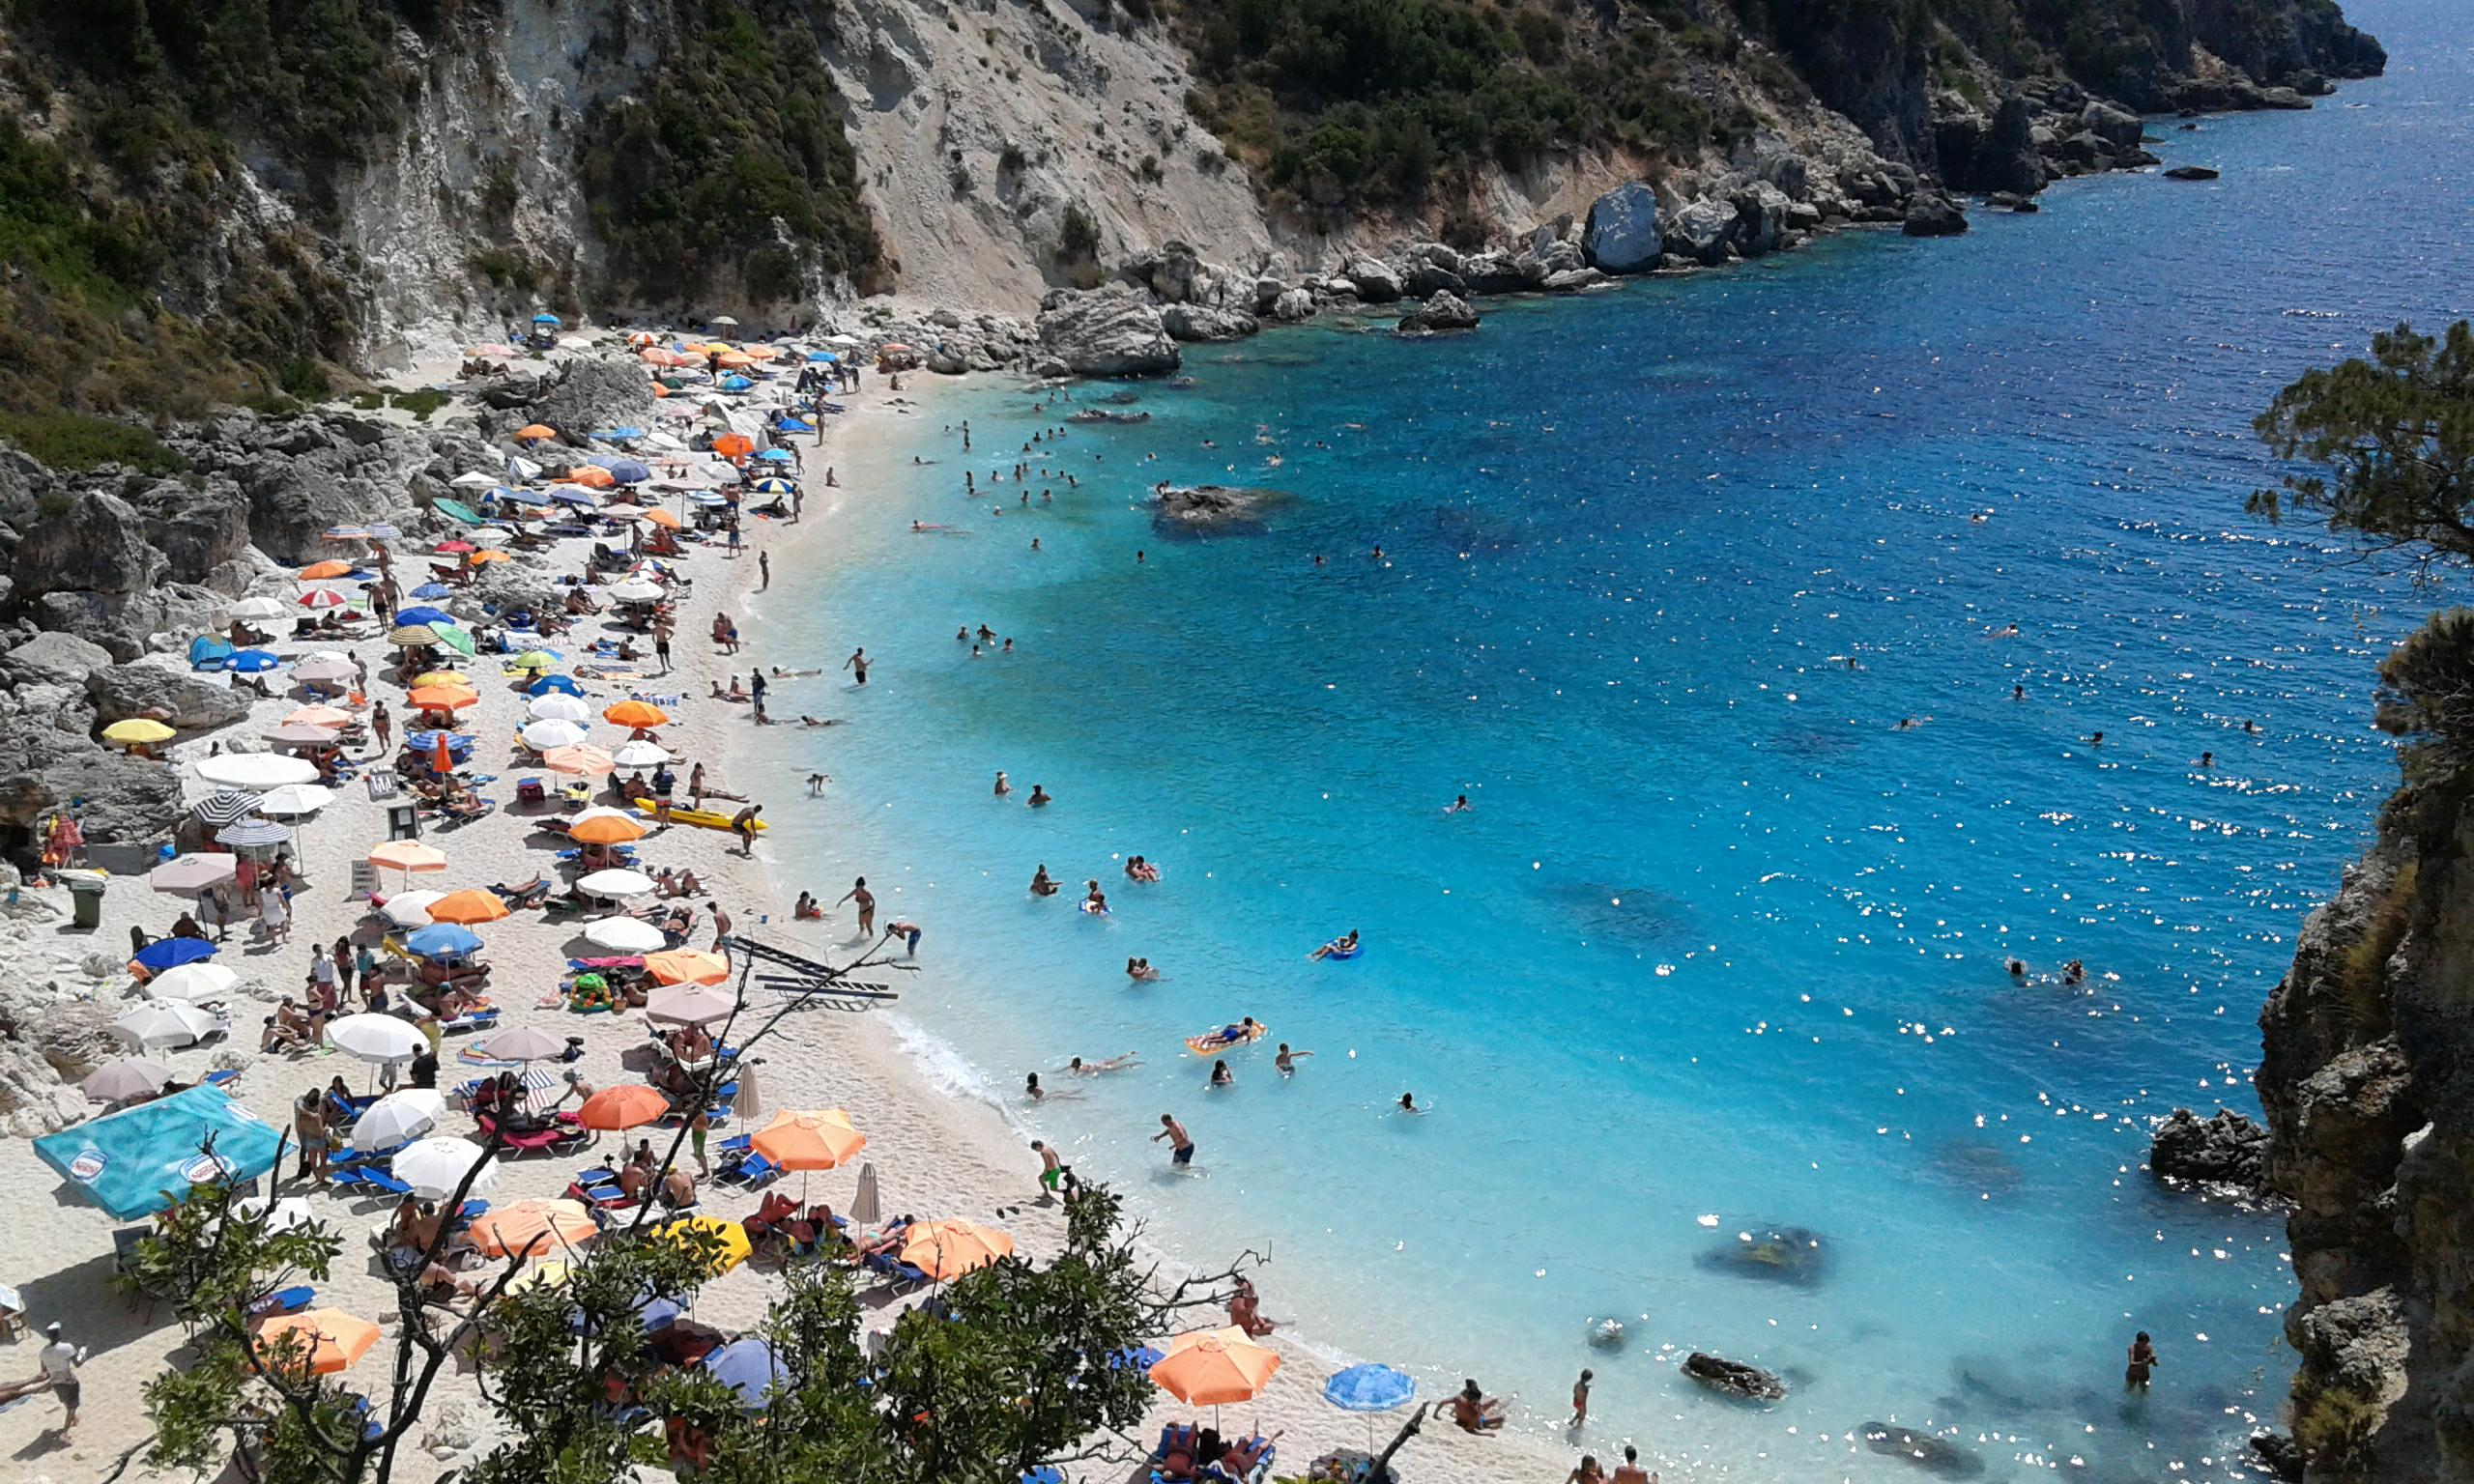
\includegraphics[width=0.32\textwidth]{media/kathisma_beach.jpg}
	\par\textit{Kathisma beach at Lefkada}
\end{center}


%1234567890123456789012345678901234567890123456789012345678901234567890123456789
My first and only visit at Lefkada's beached was at ``Kathisma''. 
Since Lefkada is on the west side of Greece it offers the possibility of 
paragliding due to the strong ``west winds''; and of course I am always up 
especially for extreme challenges. 
The particular team, of paragliding, offered two venues: i) seven minutes of flying 
from almost 300 meters, and ii) ten to twelve with fall from 600 meters. 
In addition, I was equipped with a Go Pro camera so we can capture the moment. 


%1234567890123456789012345678901234567890123456789012345678901234567890123456789
As soon as we reached the top of the hill the instructor prepared the paragliding 
equipments and attached me on it. 
On that moment, before the jump, I was not sure if I was feeling scared from the 
unknown feeling (of flying) or excited from it. 
However, as soon as we jumped (me attached together with the instructor) the 
bizarre feeling went away. 
I was feeling relax and calm, I was enjoying the unique view from the top that 
mother nature feely offered to us. 


\begin{center}
	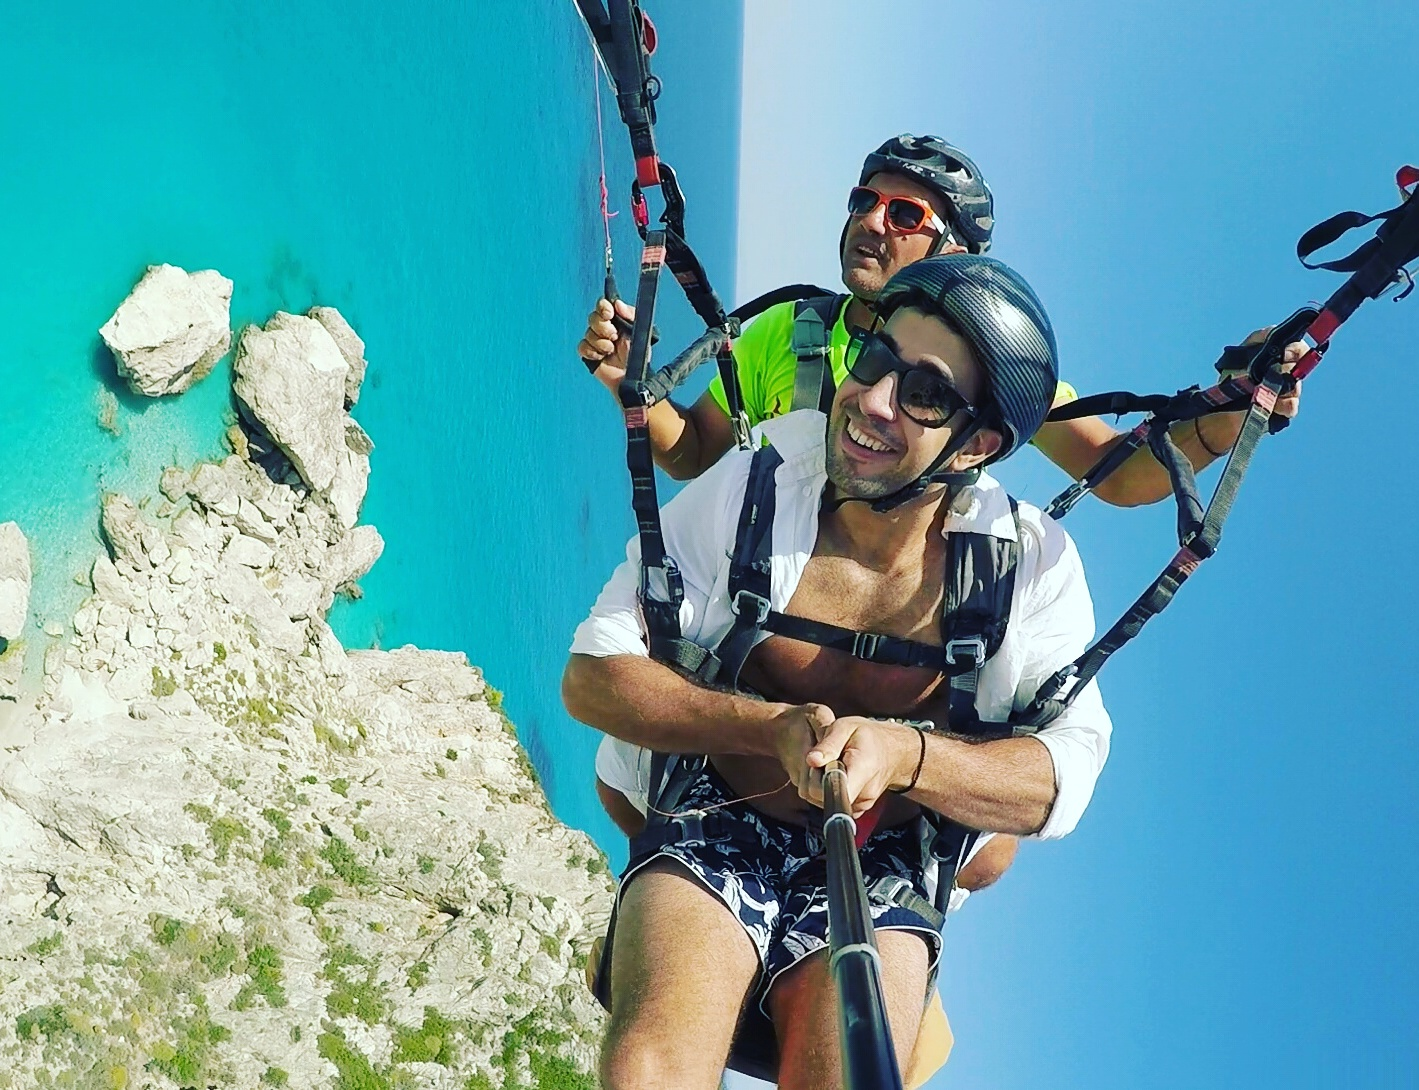
\includegraphics[width=0.32\textwidth]{media/paragliding.jpg}
	\par\textit{It is manoeuvre time!!!}
\end{center}


%1234567890123456789012345678901234567890123456789012345678901234567890123456789
Upon reaching the beach, the instructor informed my that we can have some manoeuvres 
with the paragliding, only if I wanted it, and of course I agreed on that. 
While doing manoeuvres you are losing height much faster, however, the whole concept 
was fast, immediate, and at some points I even felt that I was losing my breath. 
But I could say it was the most exciting part of the whole process and a one everybody 
should try. 


%1234567890123456789012345678901234567890123456789012345678901234567890123456789 
After the day passed and I had to take the bus back to Athens. 
The whole trip was very short but full with excitement due to the paragliding 
experience.

%----------------------------------------------------------------------------------------
\NewsItem{Camping with survival?}
% Discuss interesting stories such as Tzia and the almost dry out from water
% Moreover, discuss about Antonis screaming during the night.

%1234567890123456789012345678901234567890123456789012345678901234567890123456789
August is a month where most of the Greeks are resting and replenishing their 
batteries for the new season. 
To this end, on August 2017, we decided to have a camping experience in an island to also chill 
out and to enjoy our time on the beach. 
Our choice was Kea, a rocky and mountaineer island approximately an hour away 
from Lavrio's port.


%1234567890123456789012345678901234567890123456789012345678901234567890123456789
Our team, see picture below, composed from my PhD fellow Antonis Gkortzis 
(a beard scout boy guy, capable barman, good cold but nice humour, rum and beer addict), 
Daniela Mikeli (the girl who always smiles, jokes around, and has unlimited energy, 
and looks super cute until she starts drinking beers and watching football games), 
Marios and Maria Zacharia (the sugar couple who recently got a cute pair of twins 
and they are always up for good food and burgers).  
Antonis was our master and commander for the whole camping experience since he was 
following the tradition from his childhood. 


\begin{center}
	\includegraphics[width=0.32\textwidth]{media/the_dream_team.jpg}
	\par\textit{Me, Daniela, Maria \& Marios, Antonis}
\end{center}


%1234567890123456789012345678901234567890123456789012345678901234567890123456789
The camping side in Kea was organised, that means they had bathrooms, restaurants, 
and electricity. 
For myself, Antonis, and Daniela we had a single big tend and we had another one for 
Marios and Maria. 
Our daily schedule for the next three days included mainly activities such as hitting 
the beach, having beers and cocktails (from Antonis who is always equipped with the 
necessary barman package) and a trailing walking in the wild.


%1234567890123456789012345678901234567890123456789012345678901234567890123456789
During the first day, we where mainly chilling out on the beach since 
we arrived during the afternoon and I was also exhausted due to conference 
paper submission just a day before. 
Due to my lack of sleep I went to bed relatively early. 
However, I didn't realised that I haven't closed the tent's mosquito net all the 
way up.  
As an outcome, we all heard Antonis during the night cursing out loud while mosquitoes 
were feasting on him.  

\begin{center}
	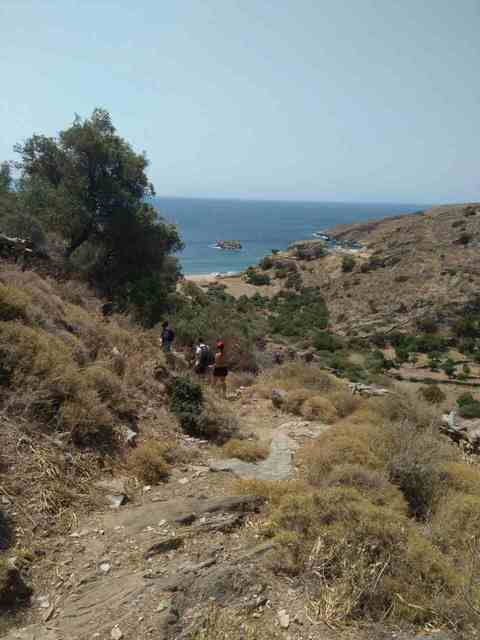
\includegraphics[width=0.32\textwidth]{media/way_to_beach.jpg}
	\par\textit{Our little adventure}
\end{center}

%1234567890123456789012345678901234567890123456789012345678901234567890123456789
As the next day's challenge, Antonis found a trail path that had as a destination 
an unorganised beach with some ancient ruins. 
According to his information the path was easy and short, around 15 minutes. 
Therefore, we started our small adventure at 10:00 o'clock in the morning. 
We arrived by cars and the old mine (that was the starting point) and we prepared 
our backpacks to start the tail. 
However, we only took three litters of water since we where expecting a short 
journey. 
Who would ever thought that the trail took us an hour to reach our destination 
that also included a rough downhill on the way?
Upon reaching our destination we run out of water and there was nothing around 
to refill our supplies. 
We were alone in the wild at an amazing beach as shown in the picture below. 
To this end, we took our time to at least enjoy the beach before we head back. 
Going back without water supplies was not only challenging but a survival task too 
since we started feeling dizzy due to dehydration.   
It took us almost an hour and a half to reach our cars where we didn't had any water 
apart from a fridge back with ice cold beers. 
That time it didn't mater us, we were  drinking them like water! 


As we made our way back to home in the next days, we were sure that the 
certain experience, of the camping and our survival in the wild, will not be 
forgotten that easy. 
As a mater of fact, we still discuss and make jokes on those events while 
drinking beers and enjoy barbecue.   


\begin{center}
	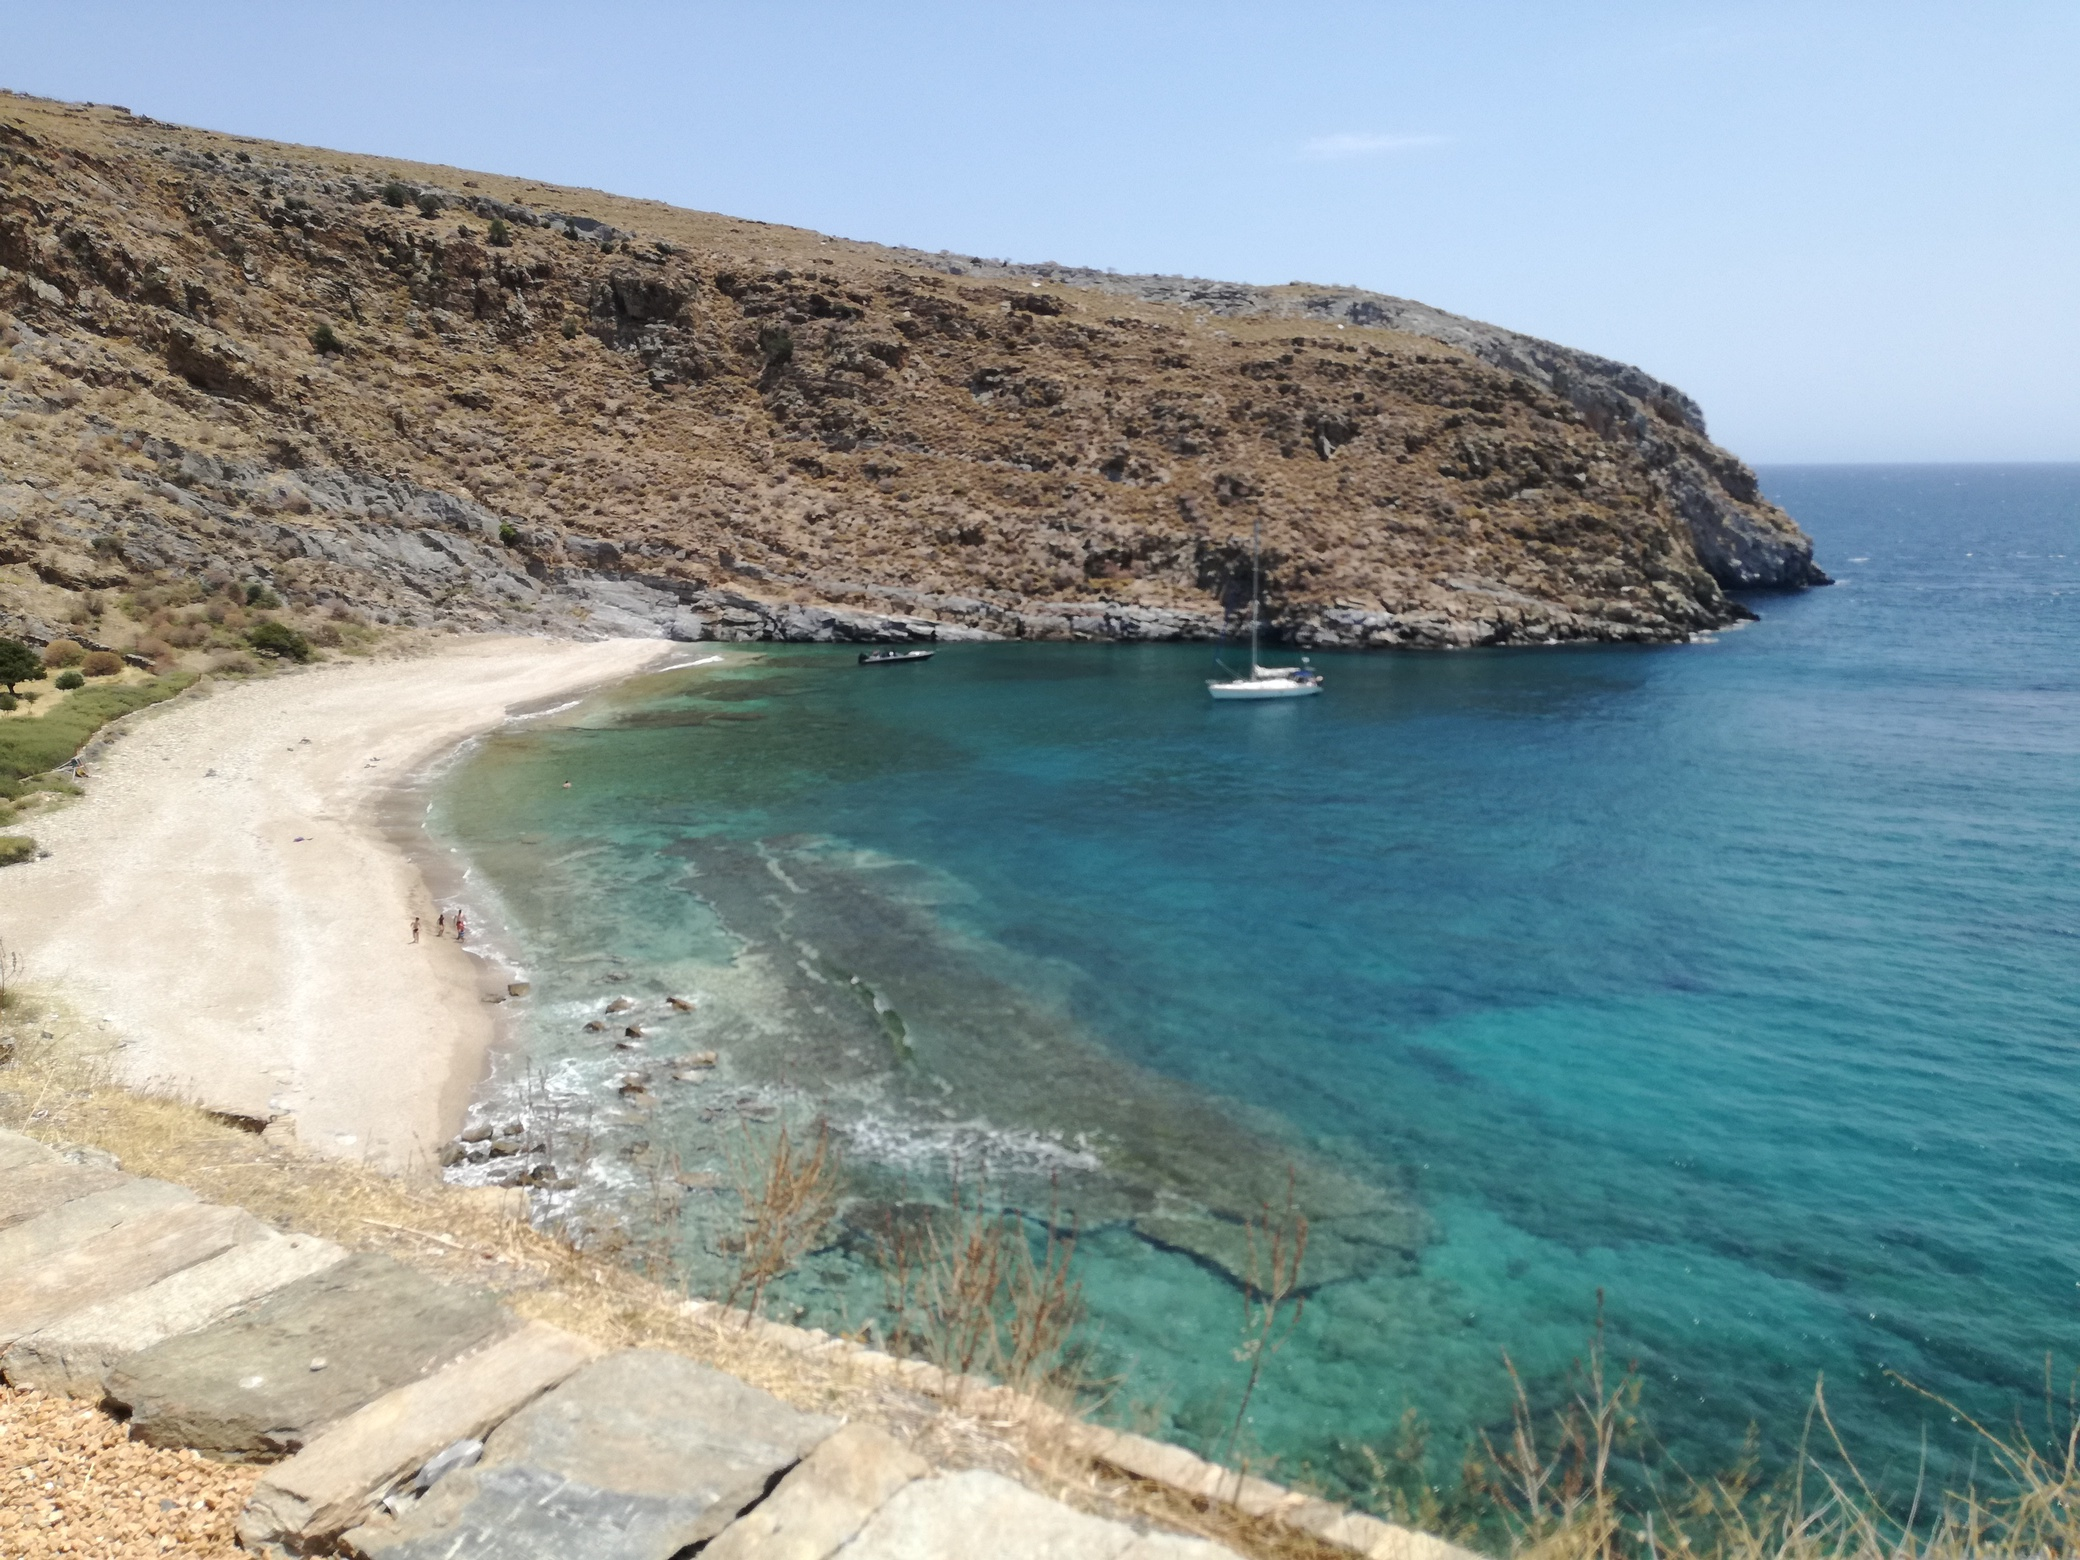
\includegraphics[width=0.32\textwidth]{media/isolated_beach.jpg}
	\par\textit{Trail walking with beach destination}
\end{center}


%----------------------------------------------------------------------------------------
\NewsItem{Can't say no to raki}
% Discuss about Chania and the driving with Alexandre De Masi in addition the 
% rakia every time that I had to drink

%1234567890123456789012345678901234567890123456789012345678901234567890123456789
Mid of August 2017, the whole Greece is on vacations, Athens looks like a ghost 
town since most of its inhabitance are on vacations. 
By that time, three friends of mine, from the masters, came to visit me. 
Our international team (a French, a Nigerian, an Indian, and a Cypriot) had aim 
of visiting Chania, one of the most tourist regions of Crete island.   
 

\begin{center}
	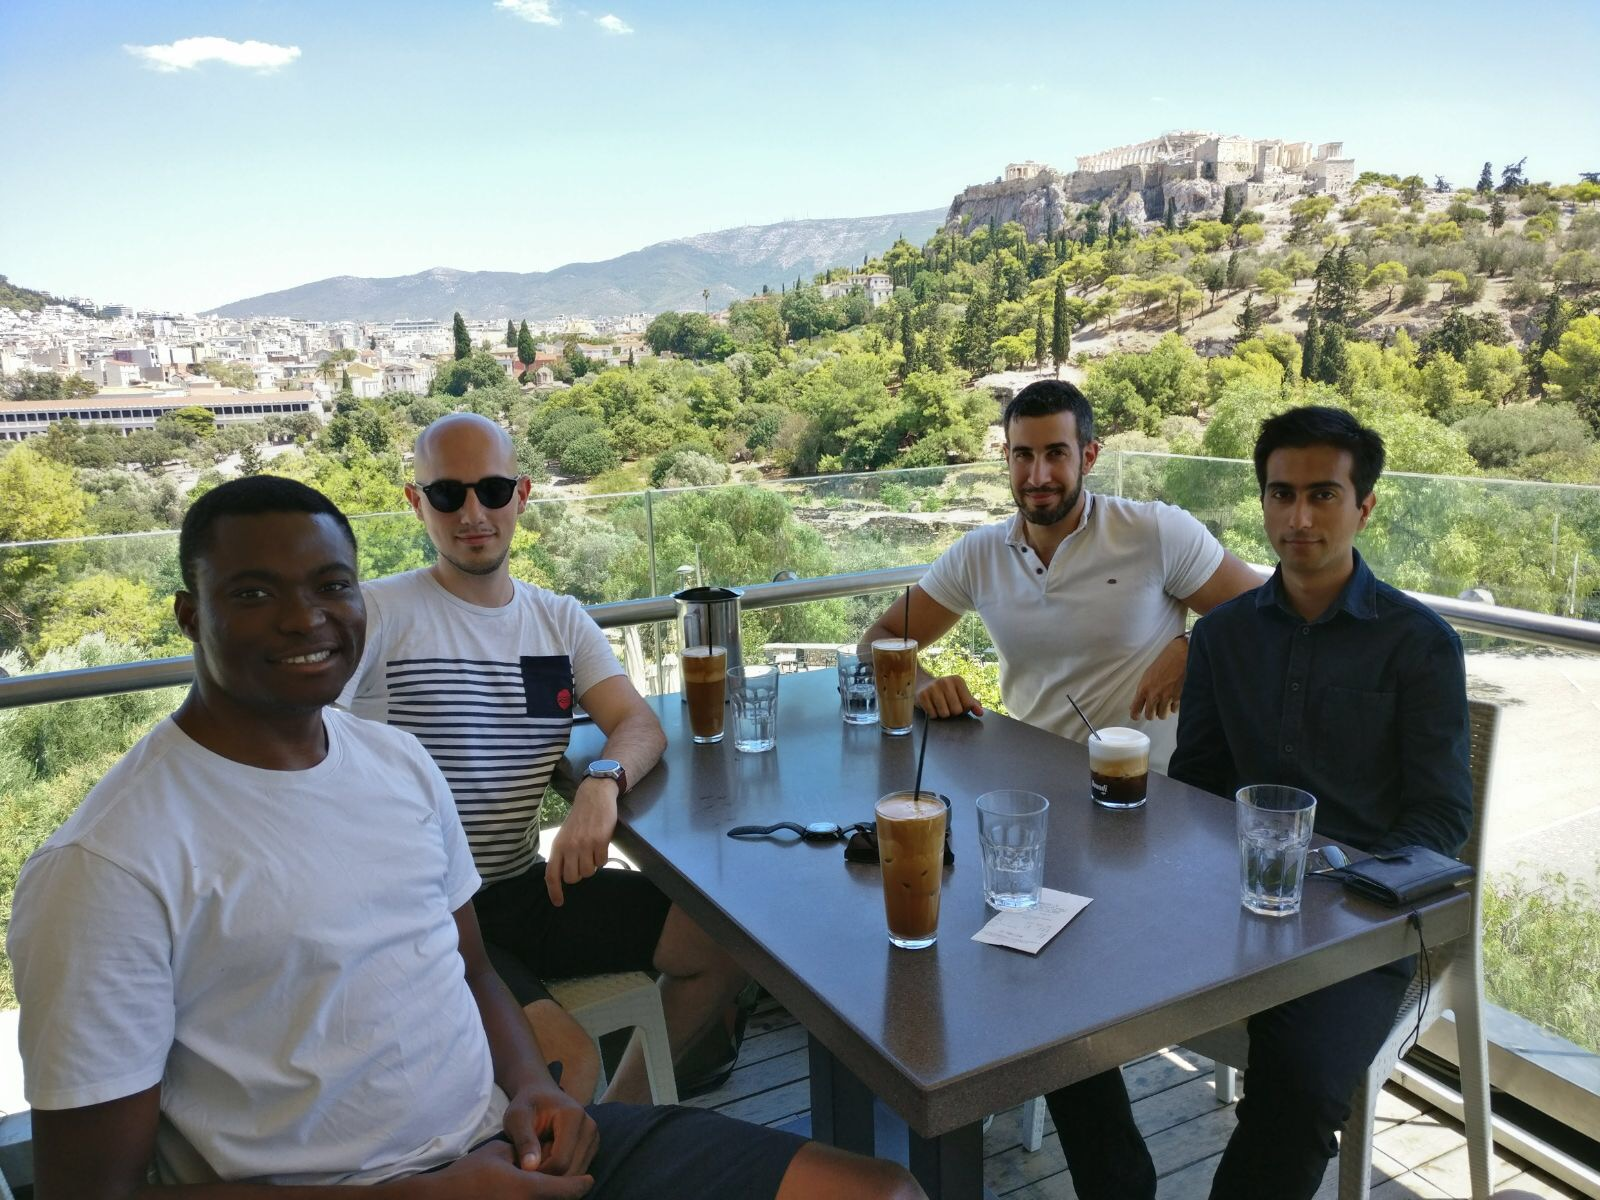
\includegraphics[width=0.32\textwidth]{media/chania_1.jpg}
	\par\textit{Fisayo, Alex, Me, and Rohan}
\end{center}


%1234567890123456789012345678901234567890123456789012345678901234567890123456789
Such a trip during August requires plan from far ahead since it is high season 
and most of places are booked in advance. 
Therefore, we made all the necessary step such booking apartments, boat tickets, 
rent a car, and prepare a plan of possible places that we would like to visit 
during our stay there. 
Since none of the guys had the boat travelling experience before, we decided 
to have reserved seats. 
However, the eight hours boat trip was indeed an exhausting decision and one 
I would most probably avoid I am not planning on reserving a cabin.  
Also, we had to choose a driver in out team, a once that could handle the 
hard and narrow streets of Crete without getting is killed. 
To choose among a Cypriot, a French, a Nigeria, and an India, for driving 
was a tough choice. 
As a rational choice seems to be me, however, in Cyprus we drive from the 
opposite side. 
Rohan didn't know how to drive and Fisayo haven't updated his driving license 
to a European one. 
Therefore, we ended up letting Alexandre the French/Italian guy to drive. 
Due to his French blood, as he said, he had to complain about every narrow and 
badly maintained street we engaged in our path. 
Despite his complain those facts he did an awesome job by giving a safe drive 
until the end of our stay in Crete. 


\begin{center}
	\includegraphics[width=0.32\textwidth]{media/seitan_limani.jpg}
	\par\textit{Seitan Limani}
\end{center}


%1234567890123456789012345678901234567890123456789012345678901234567890123456789
Among our first choices to visit was Seitan Limani. 
Towards our way to Seitan Limani, we stopped and had a lunch at the 
``Three porks''. 
A very simple restaurant, mostly for students since it is located outside 
of a University, with very delicious and cheap food. 
A fact the impressed us about Cretan cousin was the raki which was offered to us 
at very restaurant we have been, and not just a glass of it. 
Since Alexadre was our diver, Fisayo was not drinking, and Rohan had issues with his 
liver, I had to consume the raki most of the times alone. 
When we reached Seitan Limani during the afternoon it was way to crowded. 
In addition, there was not a clear path towards the beach apart from a very 
rough downhill way. 
One of those path that could easily fall and break your neck if you do not have 
wild goat's climbing skills. 
However, it did not stopped locals or tourists to go down there and enjoy its 
beautiful and refreshing blue water as depicted in the picture below. 
One of the visitor of the particular beach was a wild goat that was approaching 
people on the beach to get or snatch food from their belongings. 
Despite this, it offers an interesting sight for the tourists who also are trying 
to make selfies with goat.   


%1234567890123456789012345678901234567890123456789012345678901234567890123456789
Behind the main city's ports of Chania, one could find many hidden places and 
restaurants that are less franchised and offer the traditional flavours of 
Crete. 
You may lose the amazing view of the port, however, I believe it is worth more 
to have a better food in a much more decent price. 
Before going to Chania, I consulted a friend of mine, Ilias Dolaptsitis, 
to provide us with guidelines such as restaurants that we should visit and what 
kind of foods we must try. 
I could say I was pretty satisfied with everything we ate at Chania and especially 
with their raki that I was still consuming alone. 


\begin{center}
	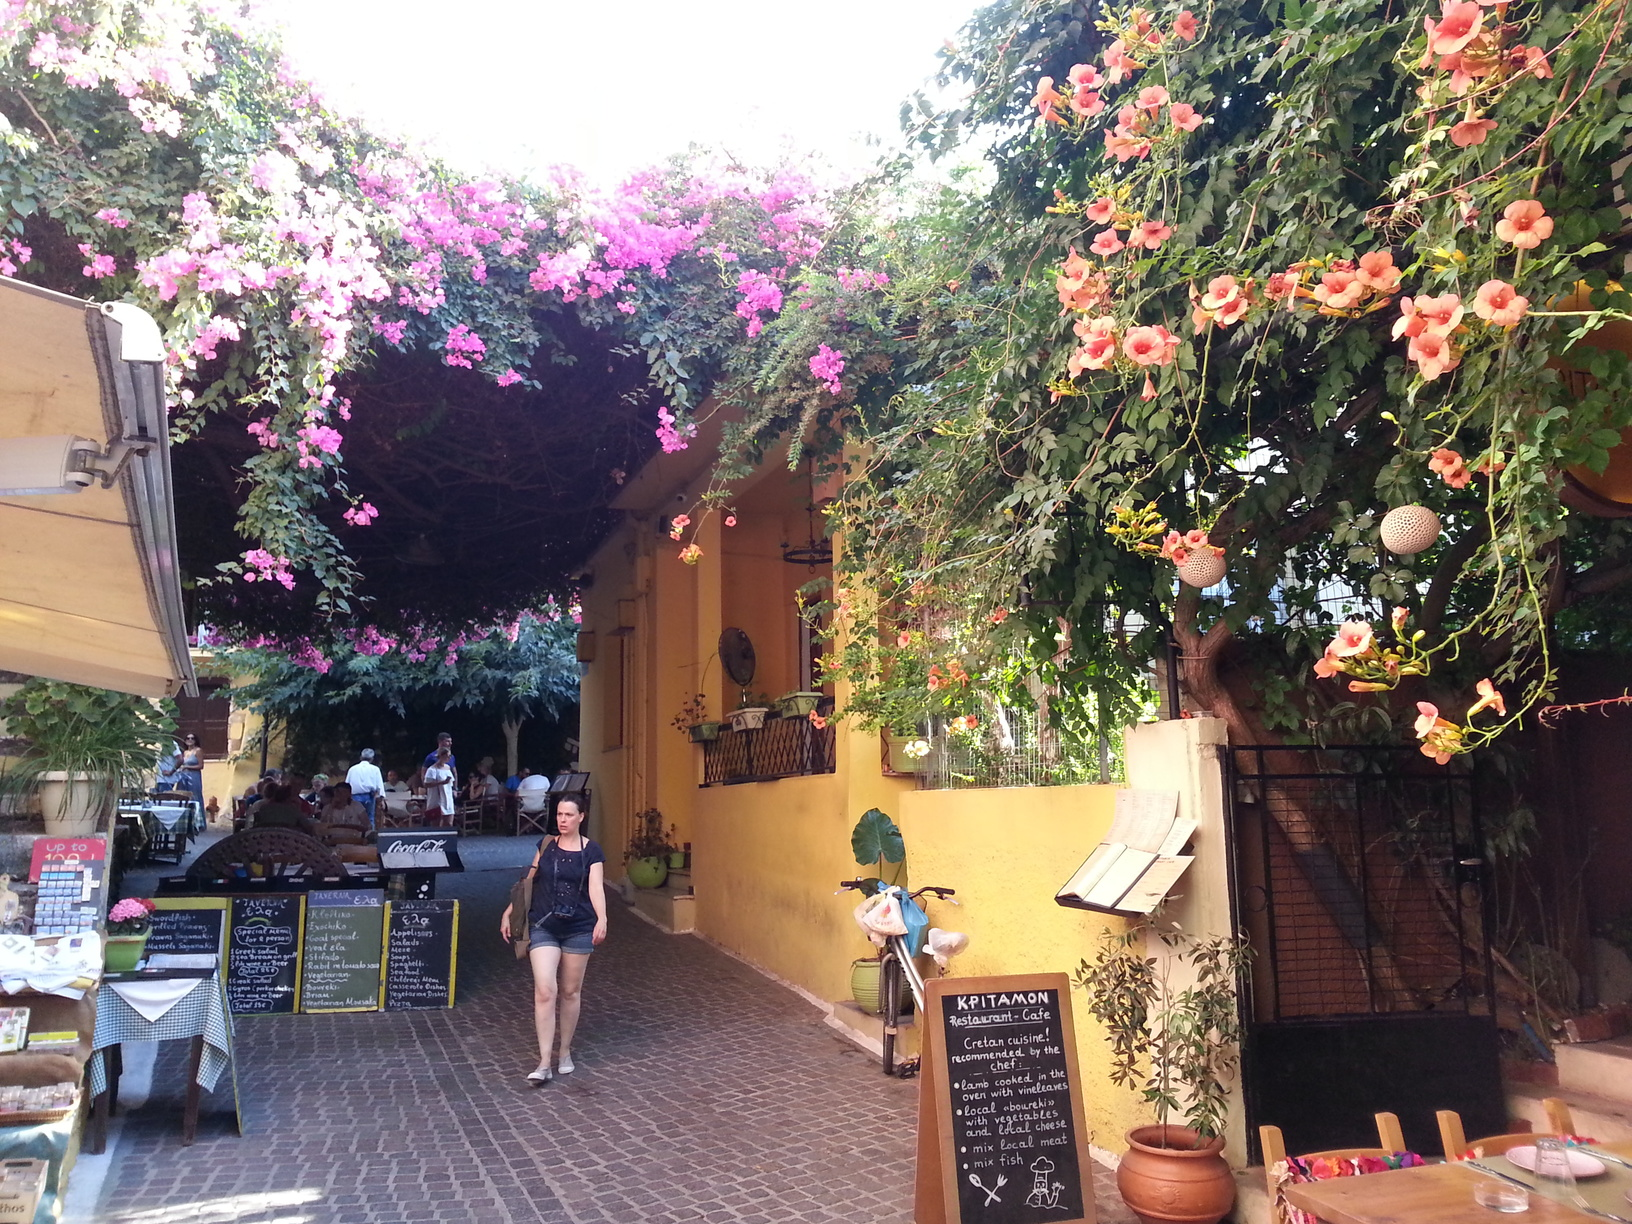
\includegraphics[width=0.32\textwidth]{media/chania_2.jpg}
	\par\textit{Hidden beauties of Chania}
\end{center}


%1234567890123456789012345678901234567890123456789012345678901234567890123456789
Driving in Crete is quite a challenge and tough task. 
It gets even more challenging when you are driving through the mountains 
where the streets much more narrow and when the buses are coming by and 
forcing you to go off-road. 
We had to go through this experience while going towards Efalonisi beach. 
However, driving trough the mountains and experiencing the beautiful environment 
of Crete paid us back for the whole straggle.



Elafonisi beach is just imaginary, beautiful white sand and crystal clear water 
can be found all along the cost-line. 
In addition, at some parts pink and black sand exist which provides a spectacular 
view while combined with sea's blue colour.


\begin{center}
	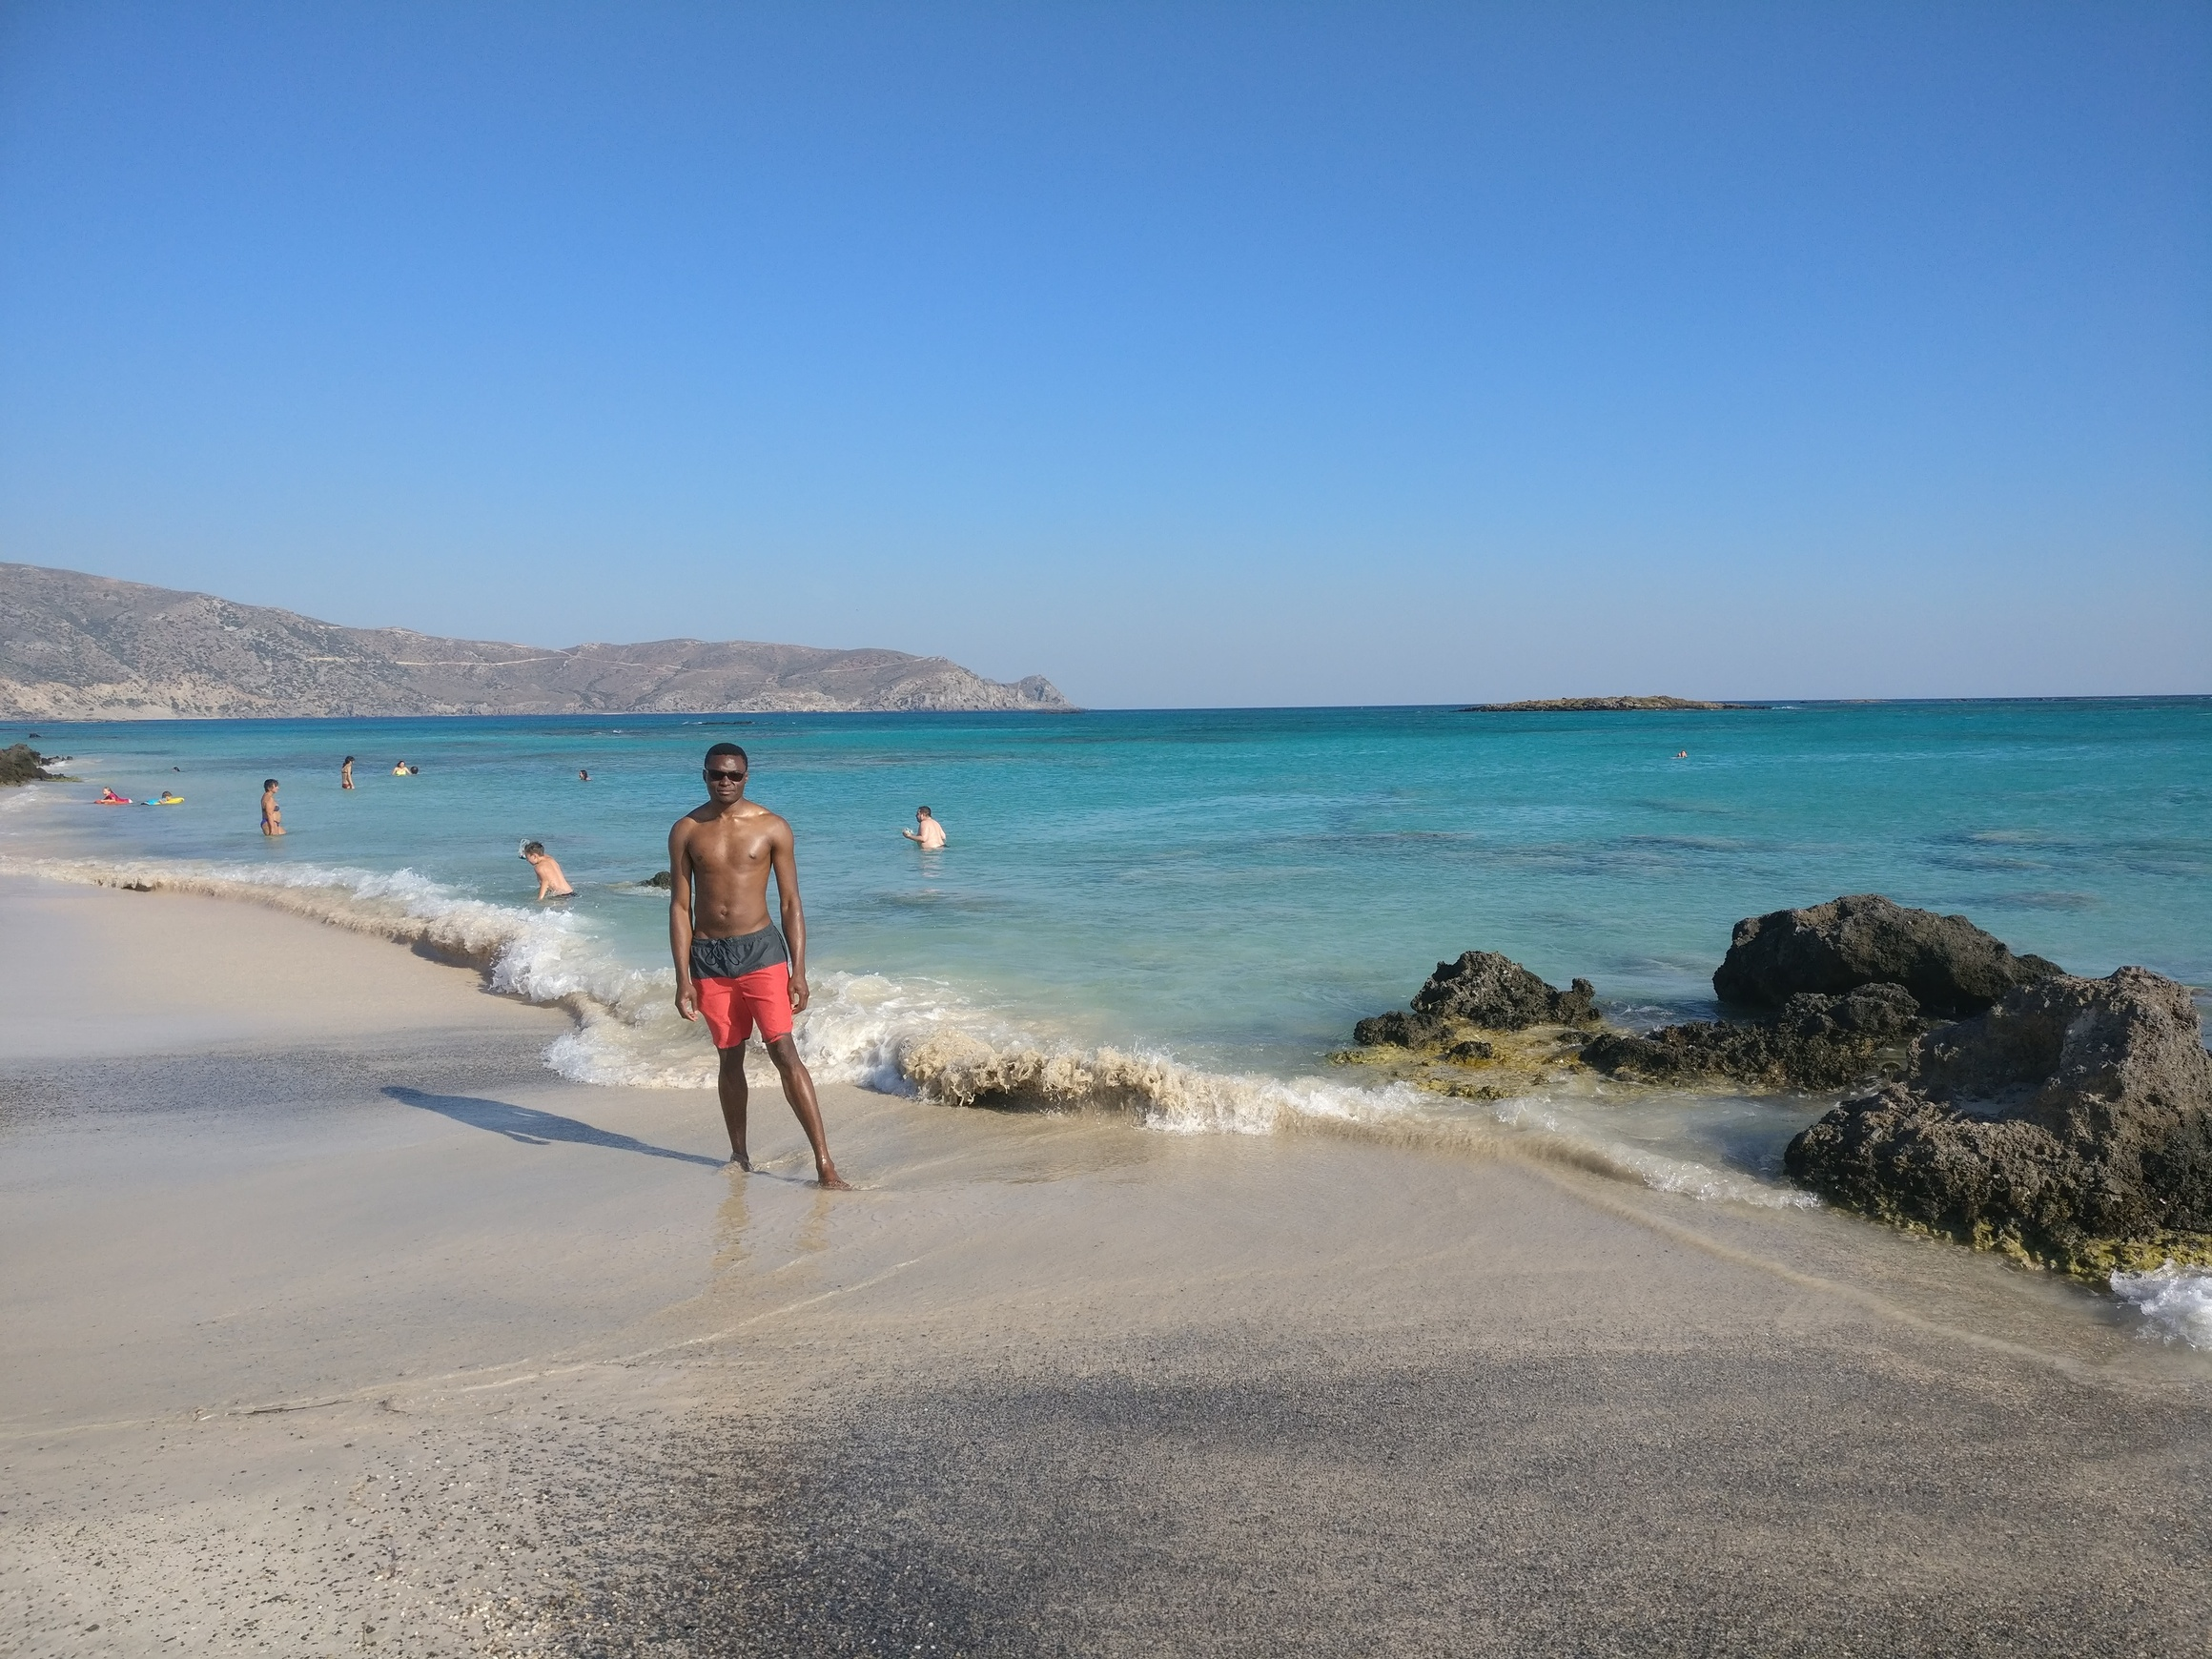
\includegraphics[width=0.32\textwidth]{media/elafonisi}
	\par\textit{Fisayo posing at Elafonisi beach}
\end{center}


%1234567890123456789012345678901234567890123456789012345678901234567890123456789
Also, Elafonisi is among the most popular touristic attractions for Chania as it is considered 
one of the most beautiful beach of Crete. 
The beach is partially organised offering all the convenience for the tourists and 
locals. 
The road towards Elafonisi was tiresome and cumbersome but the view of the beach 
at the end was charming and magazining us to stay for longer. 
However, driving during the night through the mountains was out of question!

%1234567890123456789012345678901234567890123456789012345678901234567890123456789
\begin{center}
	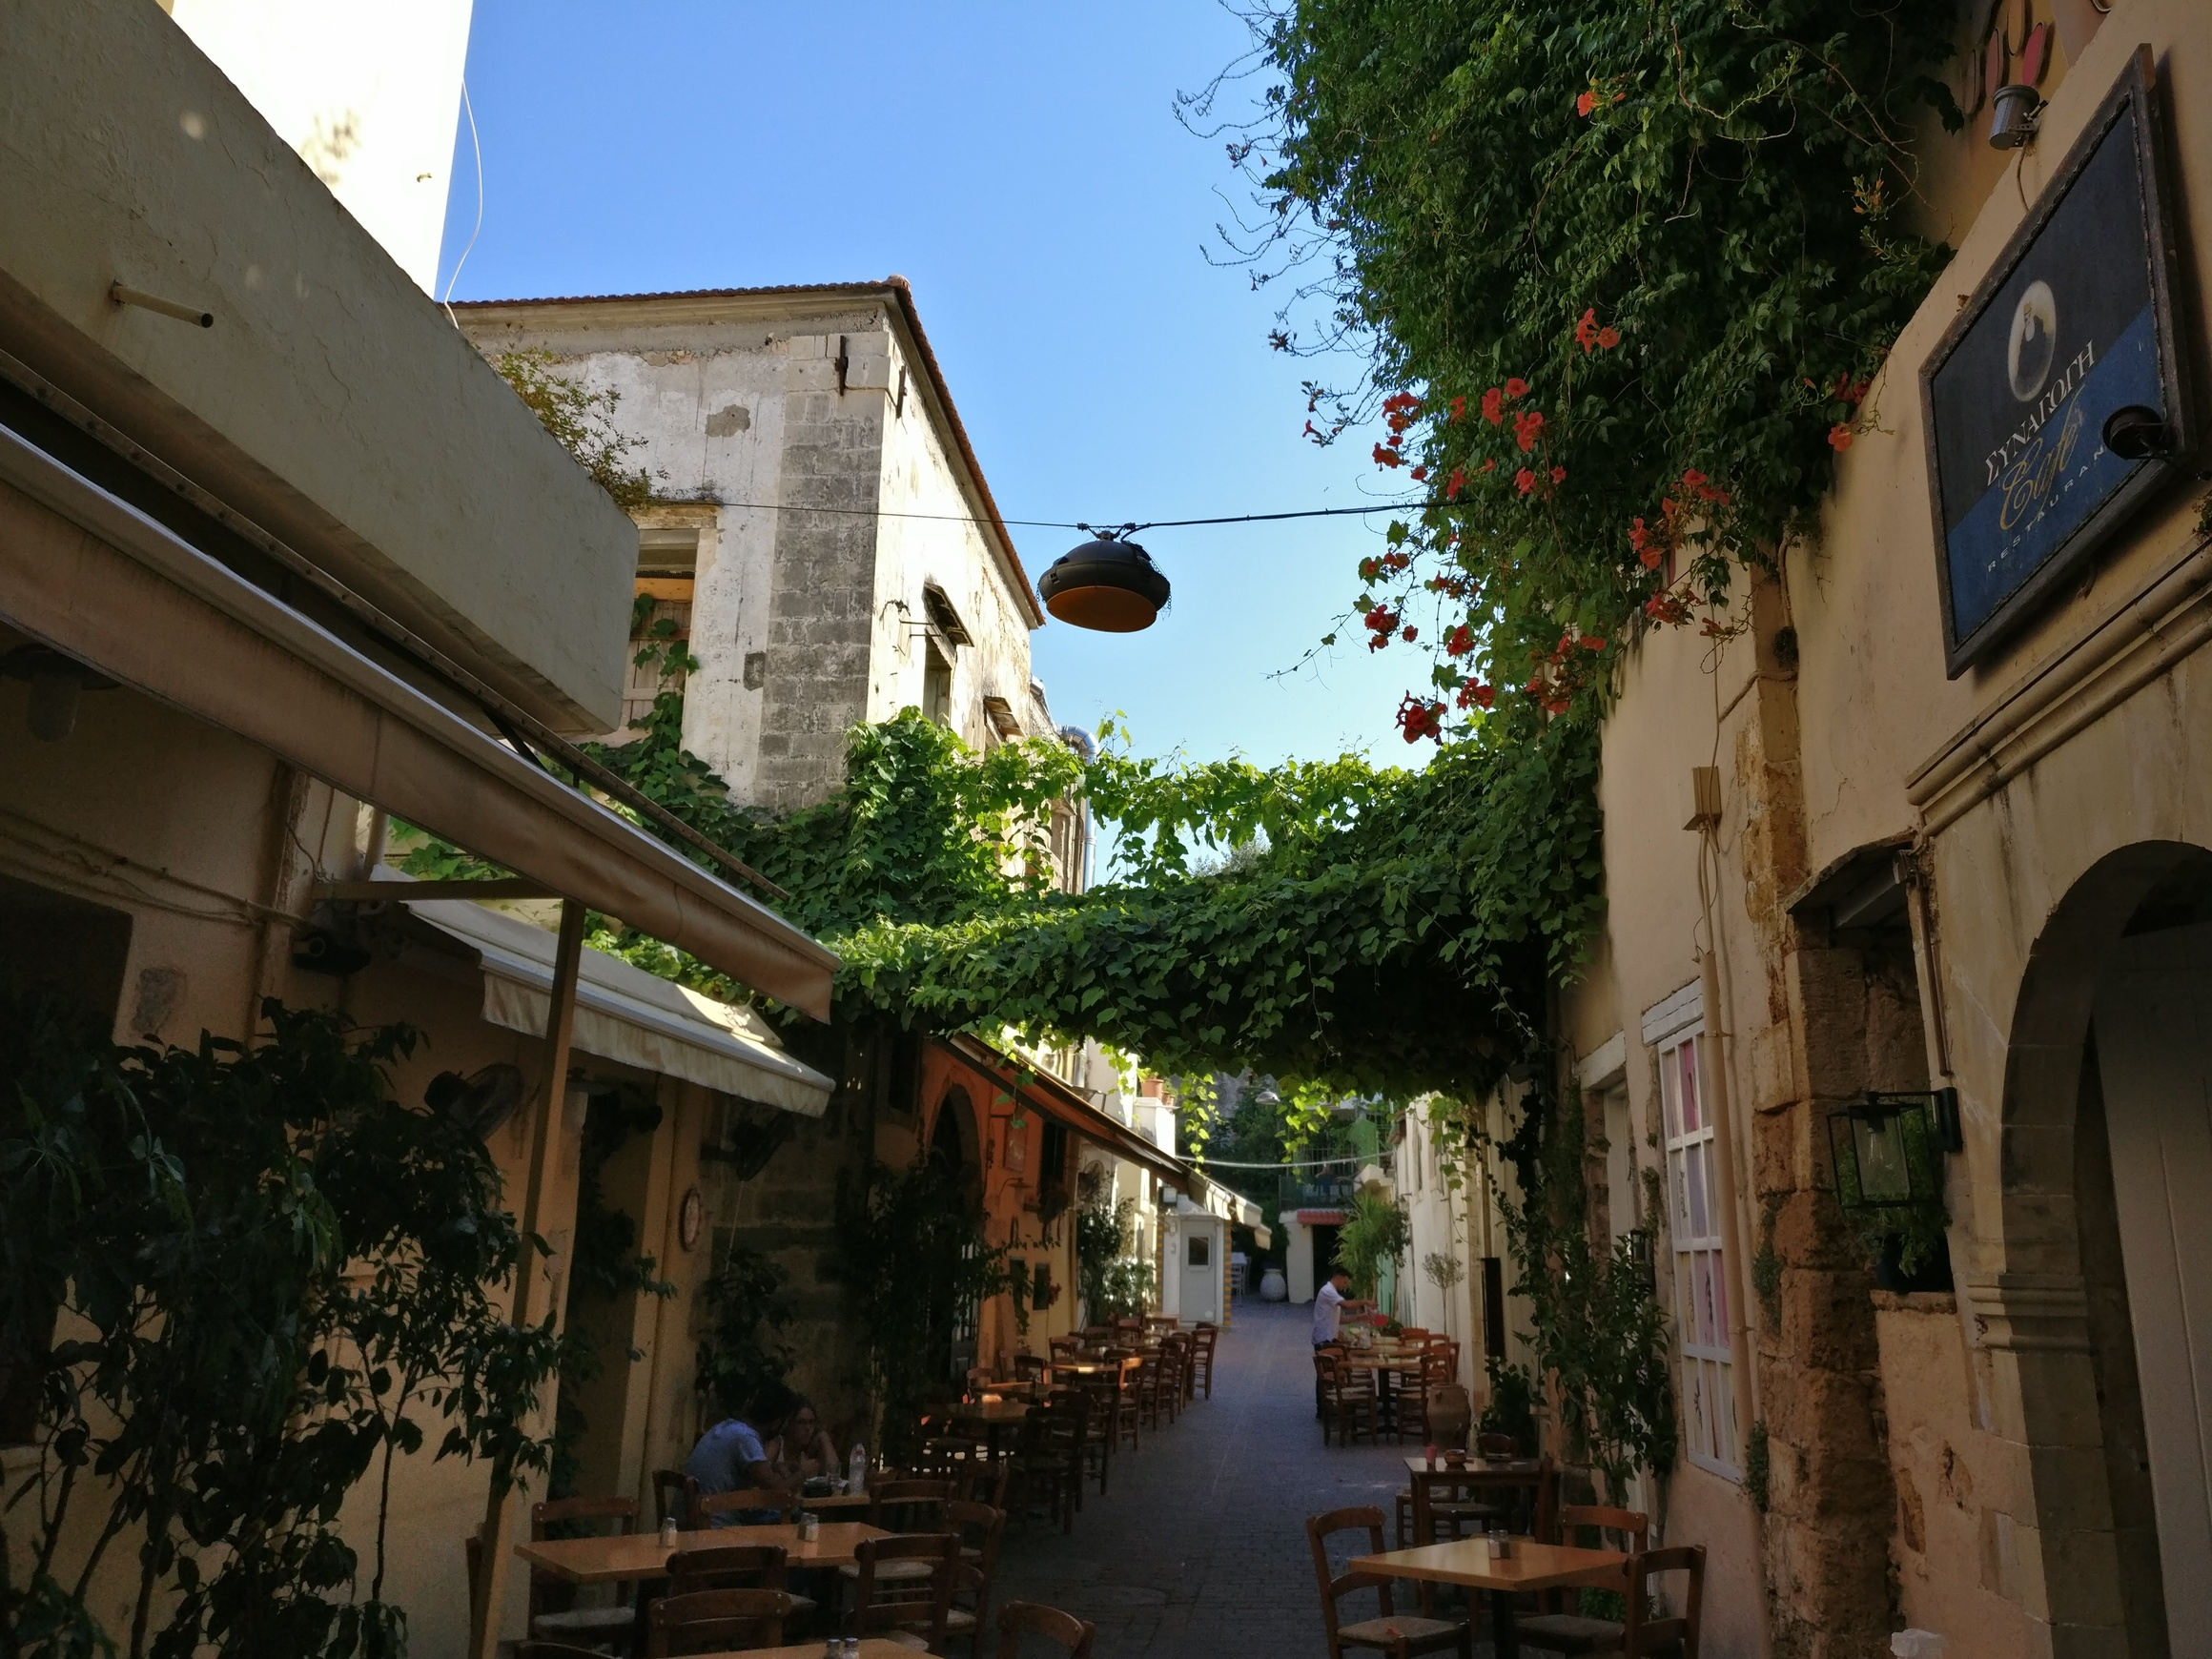
\includegraphics[width=0.32\textwidth]{media/chania_3.jpg}
	\par\textit{Parts of the old city}
\end{center}



%----------------------------------------------------------------------------------------
\NewsItem{Small but beautiful Agkistri}

%1234567890123456789012345678901234567890123456789012345678901234567890123456789
After coming back from Chania, with the international team, Rohan and Alexandre 
had to leave. 
Therefore, me and Fisayo, we decided to have one more little adventure by travelling 
to very small island just next to Aigina, the Agkistri. 
Agkistri's direct translation is the ``fishing hook''. 
To this end, we took a boat from Pireaus early morning and after an hour we 
reached our destination.


%1234567890123456789012345678901234567890123456789012345678901234567890123456789
As soon as we disembarked at Agkistri's port, we rented two bicycles. 
I really enjoy cycling in the islands when they are not mountaineer since it 
releases childhood memory of freedom.  
Since it was my first time at Agkistri we asked local for information such as 
the best restaurants and beaches to visit. 
People mostly suggested us to visit the Chalikiada beach. 
Therefore, we made our way there while cycling next to the seaside and enjoying 
the beautiful view as illustrated below.
 

%1234567890123456789012345678901234567890123456789012345678901234567890123456789
\begin{center}
	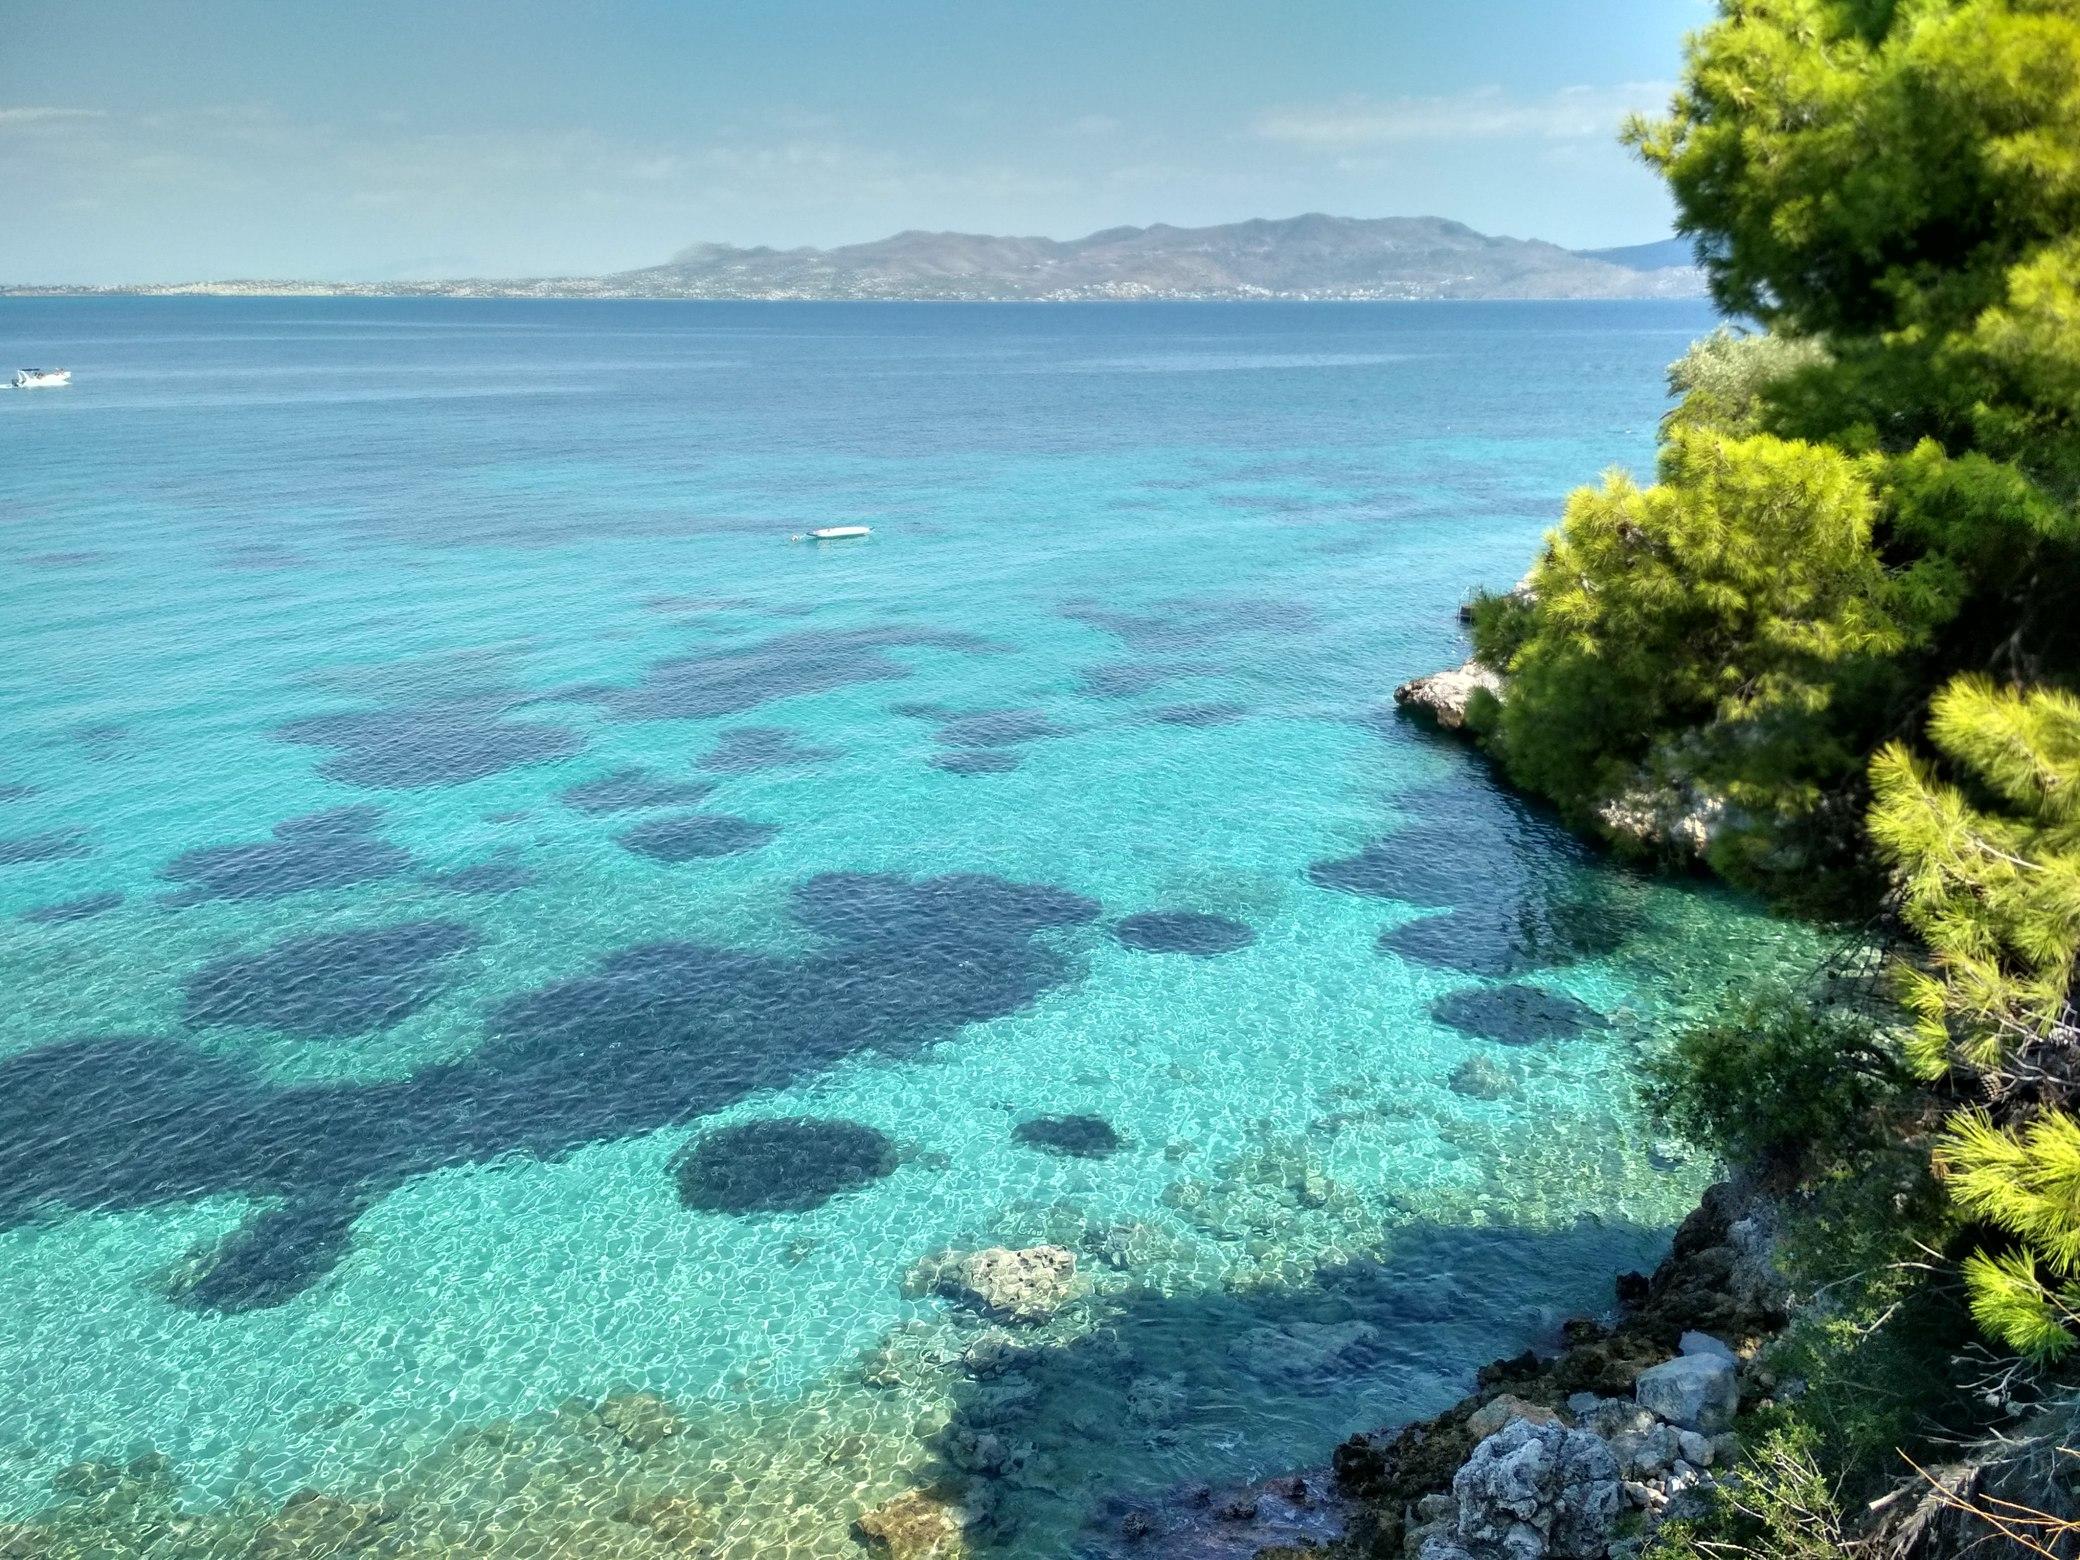
\includegraphics[width=0.32\textwidth]{media/agkistri_beach}
	\par\textit{Those amazing colours...}
\end{center}


%1234567890123456789012345678901234567890123456789012345678901234567890123456789
Chalikiada is a nude beach at the north west part of the island and ``hidden'' from 
the public (this is what we said after we passed the same road 3 times until we found 
the passage towards the beach).  
The beach is only accessible by food along side the sea through the camping area 
that is populated during summer since it is for free. 
Along the way to the beach there are many apartments with direct view to the sea 
and multiple small islands located around Agkistri, the perfect sport for 
romantic dates and love birds.


\begin{center}
	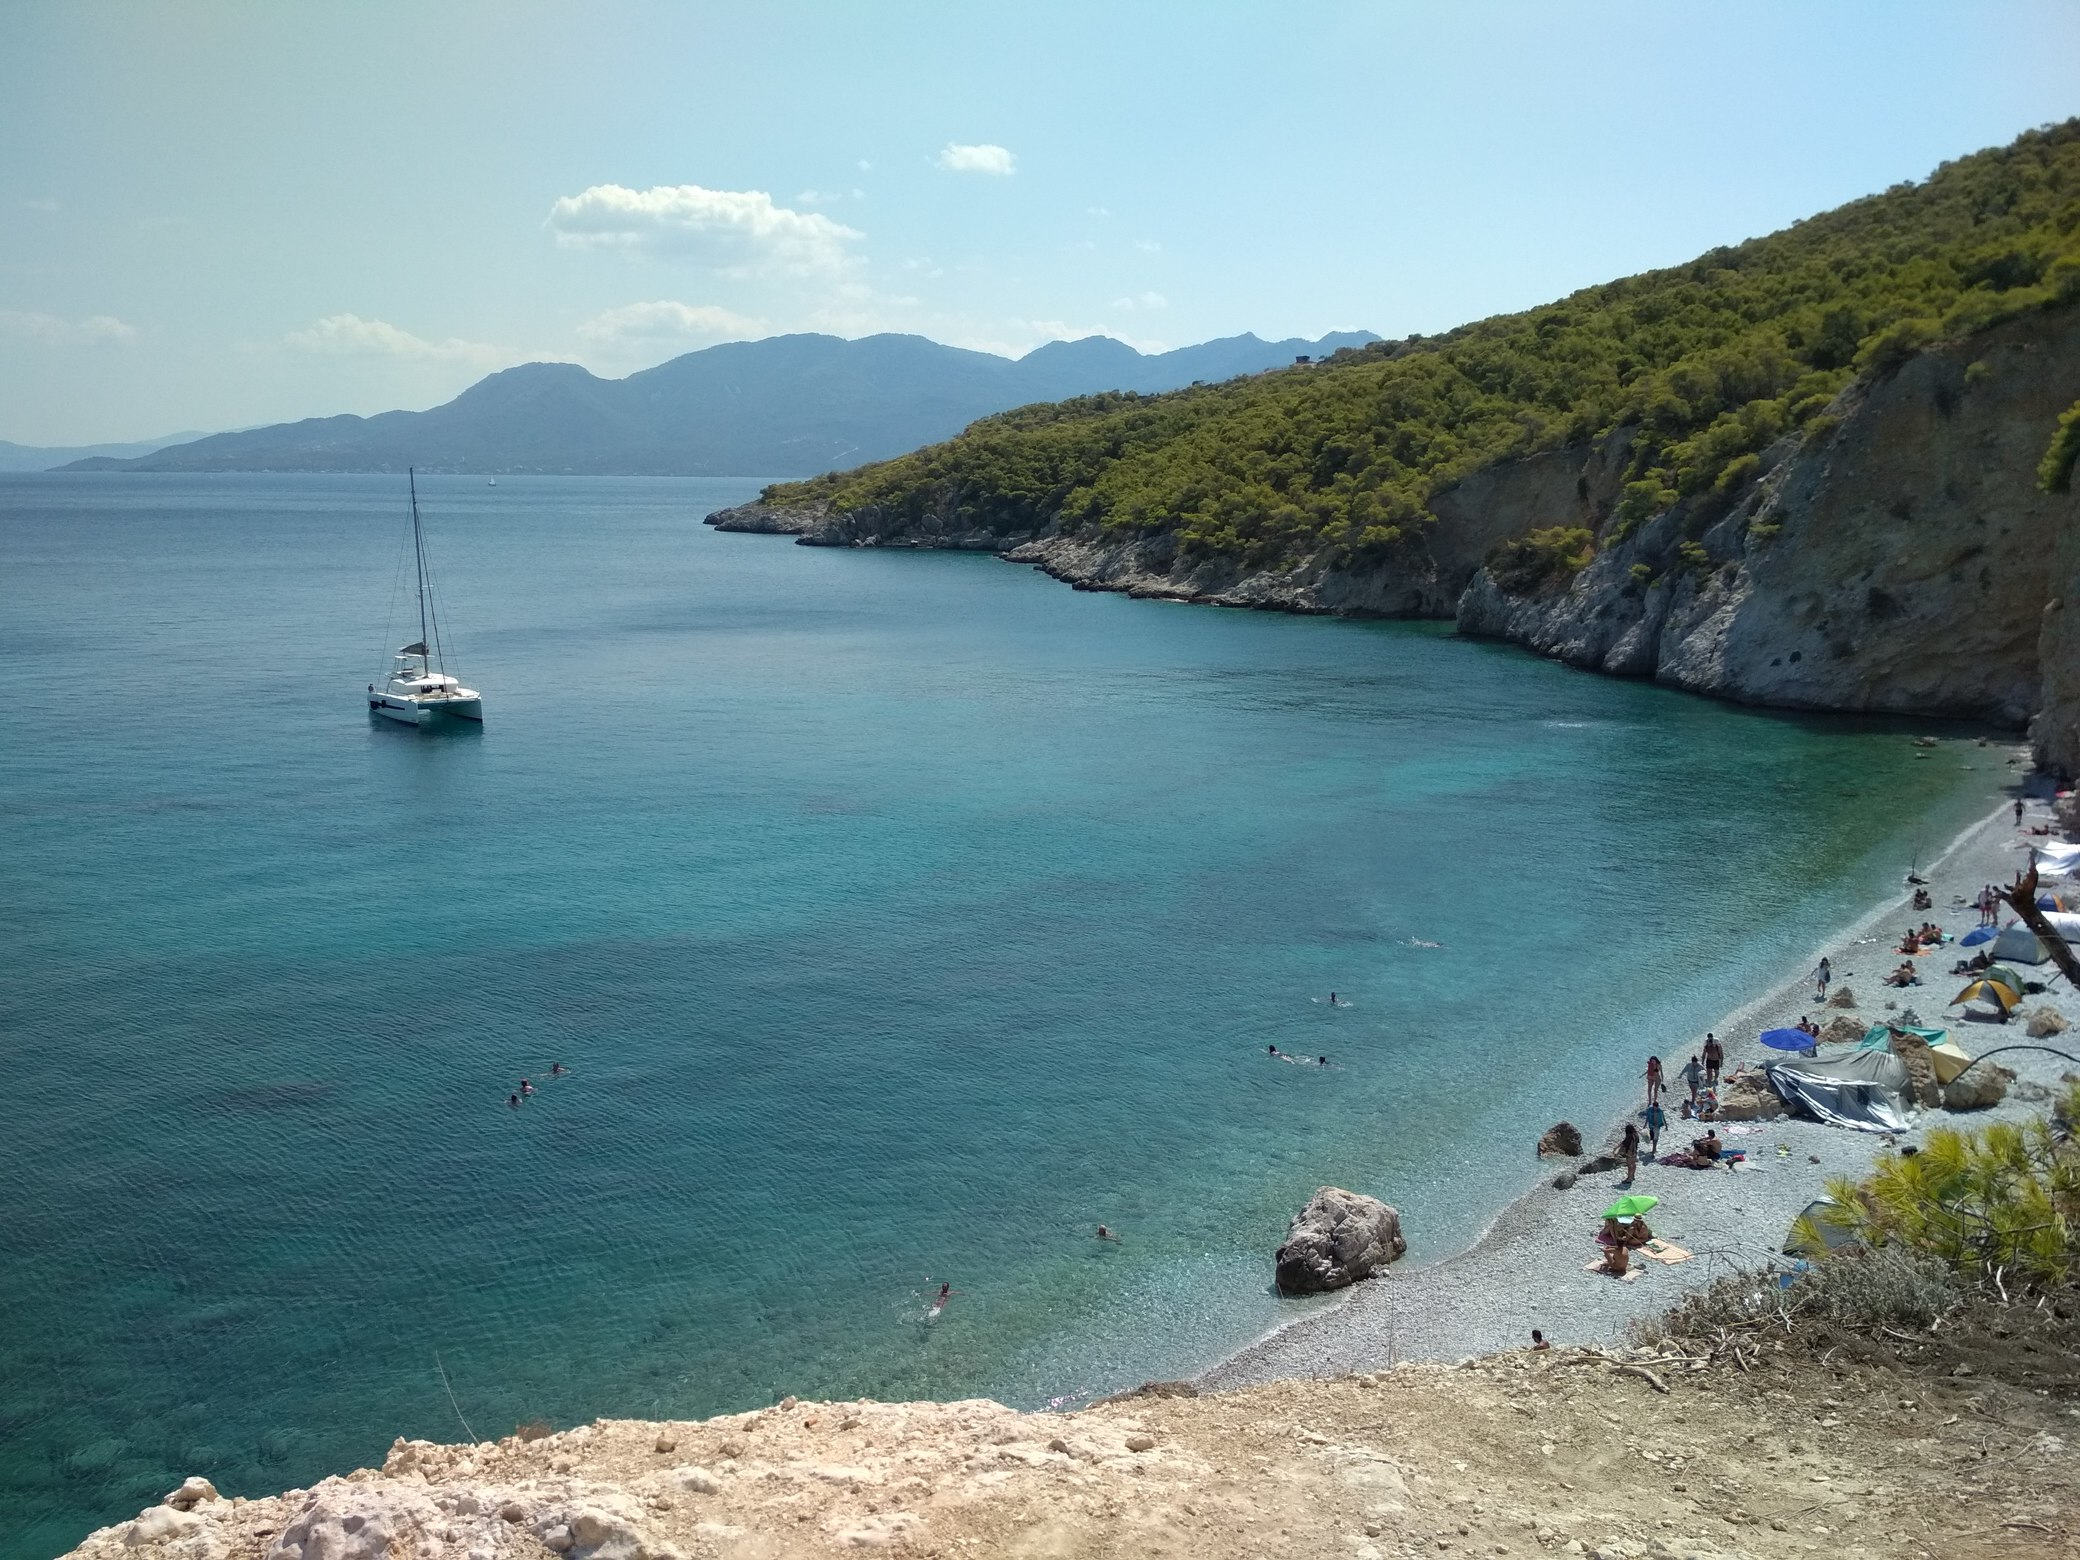
\includegraphics[width=0.32\textwidth]{media/chalikiada_beach}
	\par\textit{The beach of Chalikiada}
\end{center}


%1234567890123456789012345678901234567890123456789012345678901234567890123456789
Before the sunset, we started heading back. 
Next to the port, a nice cafeteria exists where you can have beautiful view 
towards Sarronic and you can, somehow, enjoy the sunset before taking the ship 
back to Pireaus.


%----------------------------------------------------------------------------------------
\NewsItem{Hydra, no cars allowed}

%1234567890123456789012345678901234567890123456789012345678901234567890123456789
% Speak about the heroes of Hydra like Kanaris?

Some Greek islands have restrictions to cars and motor bikes, those are the islands 
I call ``no-noisy-irritating islands''. 
After staying too long in Athens, where a majority of cars and motor bikes are modified 
just to be more noisy, the necessity of getting away from this mess is huge. 
Therefore, such islands as Hydra where the transportation is only done by feet and 
donkeys do exist. 


%1234567890123456789012345678901234567890123456789012345678901234567890123456789
By the September 2017 a friend of mine, Dorine Petit from France came for a 
conference meeting in Athens with her boyfriend Jeremy, and since they 
never been to an island before we decided to visit Hydra. 
Hydra is a large mountaineer islands just an hour and a half away from Pireaus 
port. 
It has one of the most beautiful city port that I ever seeing. 
However, its beaches, the ones that we visited, are mainly rocky.  

\begin{center}
	\includegraphics[width=0.32\textwidth]{media/hydra_port}
	\par\textit{The port and main city of Hydra}
\end{center}


%1234567890123456789012345678901234567890123456789012345678901234567890123456789
Since it was my first time and I haven't took any information from friends 
regarding places to visit of restaurants to eat, we followed the rule of thump 
``go where you see the most locals''. 
Usually going to restaurants which are mostly populated by locals it indicates 
good quality of food and value for money. 
To this end, we end up at \textbf{[...]}


\begin{center}
	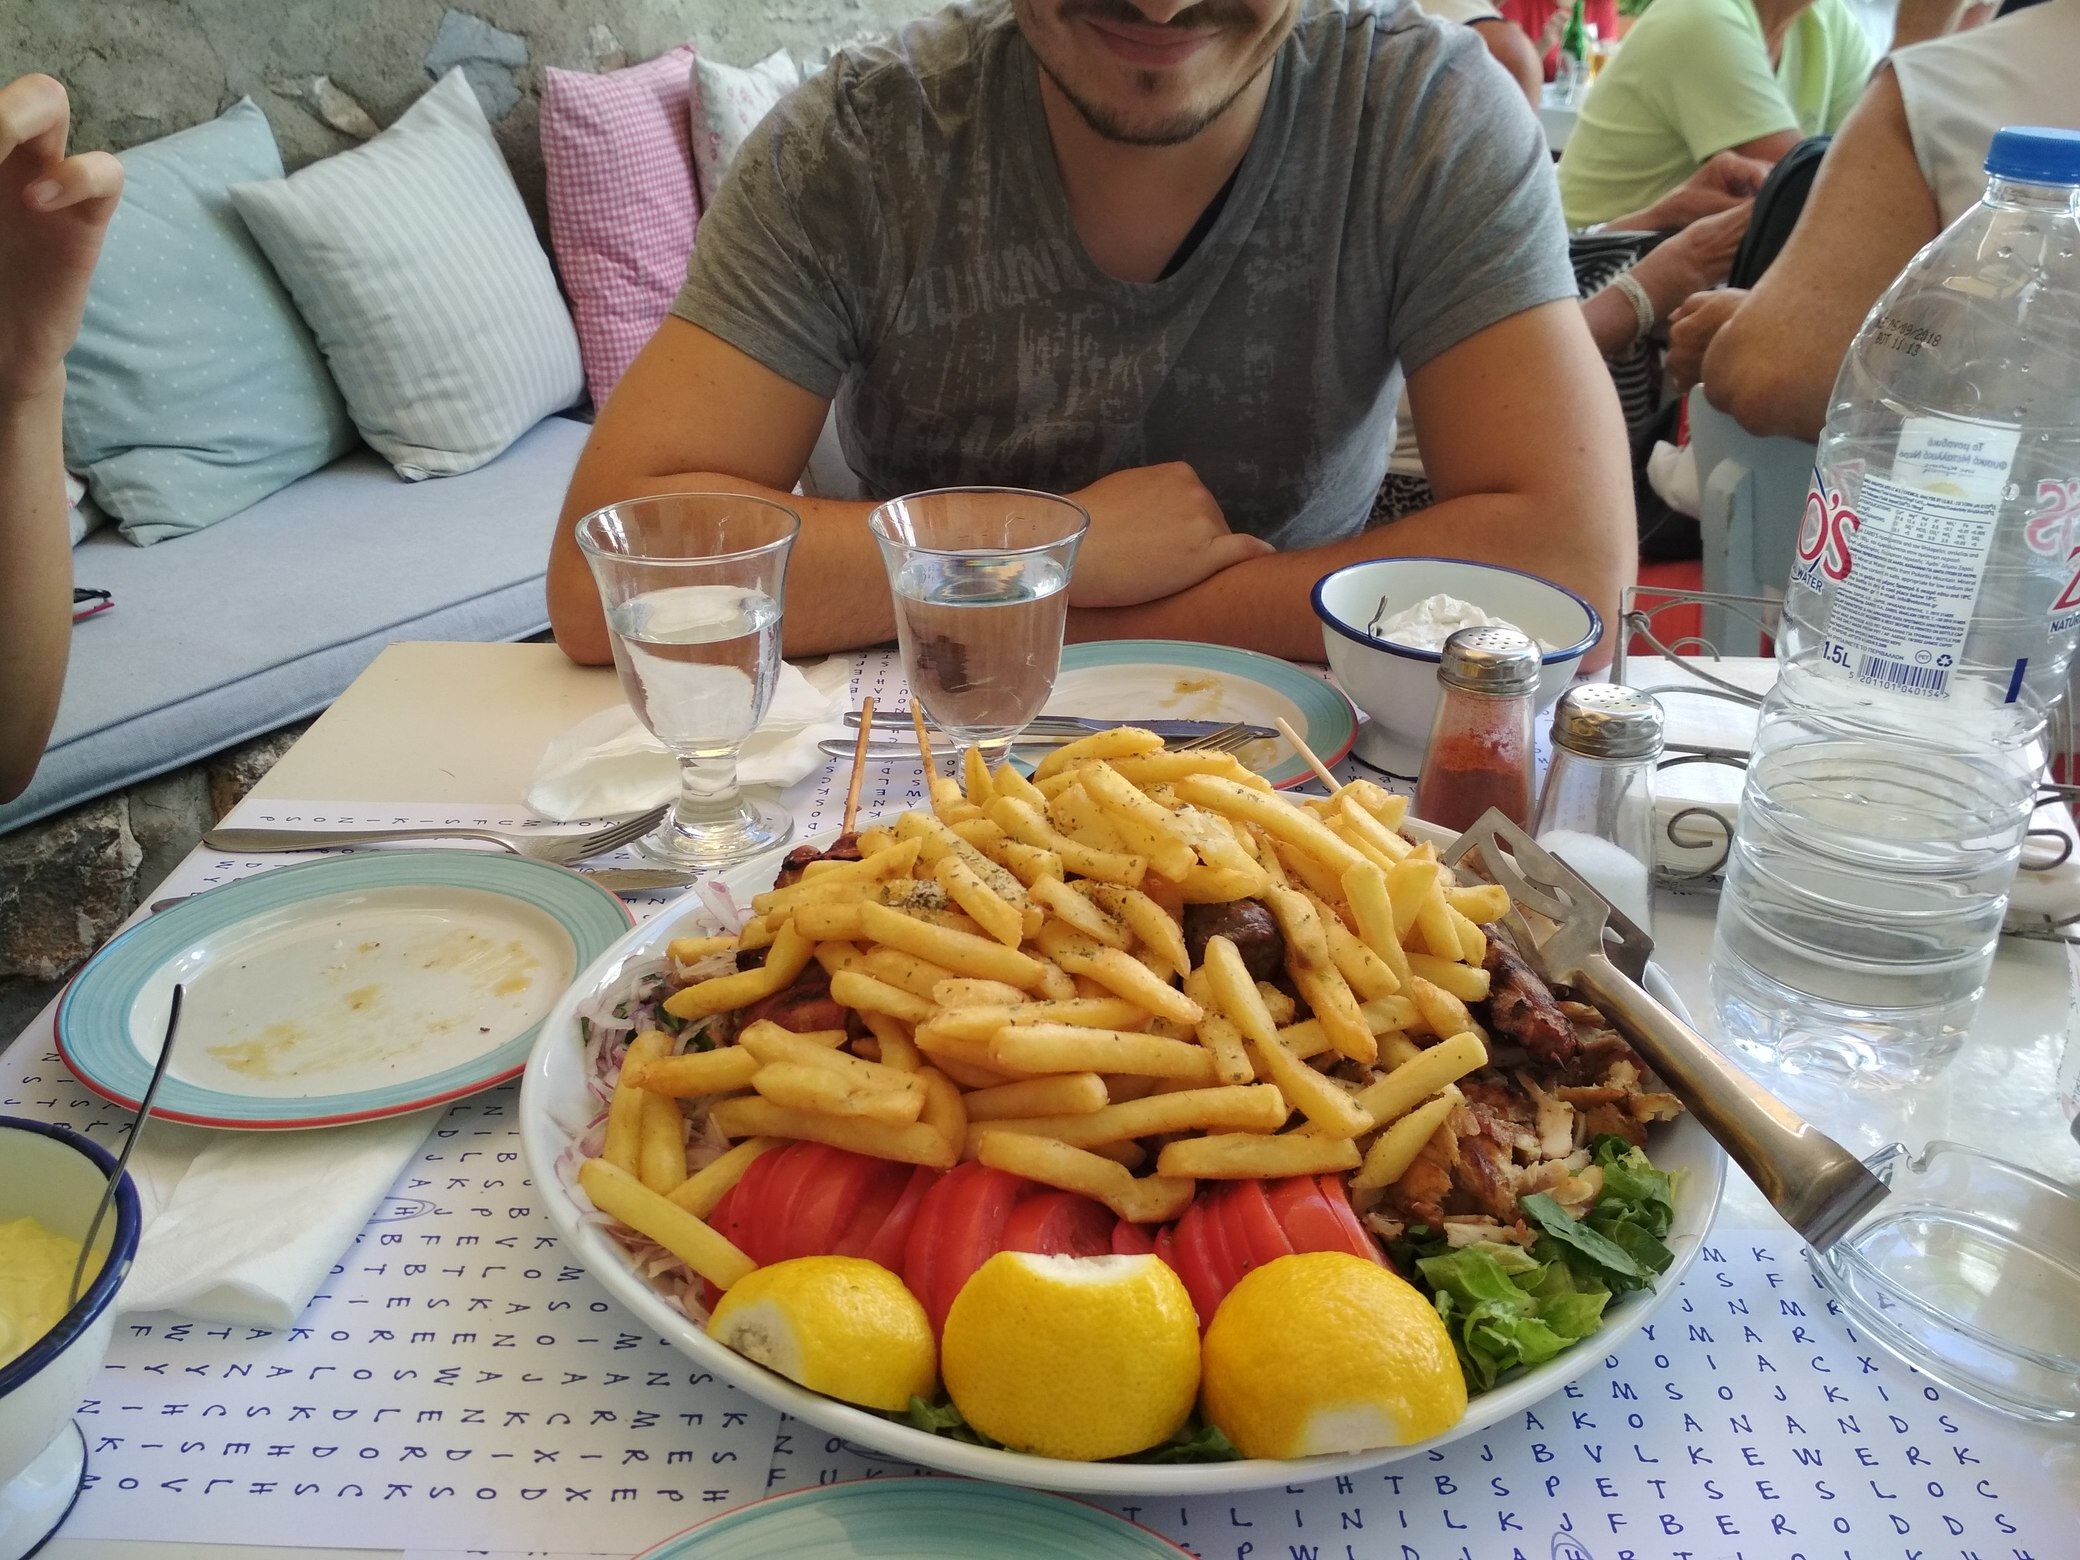
\includegraphics[width=0.32\textwidth]{media/hydra_food}
	\par\textit{Amazing mixed grill plate}
\end{center}


%1234567890123456789012345678901234567890123456789012345678901234567890123456789
To reach the beach \textbf{[NAME OF THE BEACH]}, that locals informed us, 
we had to walk 20 minutes all along the coat line of the island and passing 
through small settlements of the locals. 
The beach was mostly rocky with few brown sand. 
Also, the water had very nice temperature considering the fact that it was 
end of September. 
Dorine and Jeremy really had great time enjoying the water, the sun tanning, 
and the traditional Greek cold coffee, the frappe. 


\begin{center}
	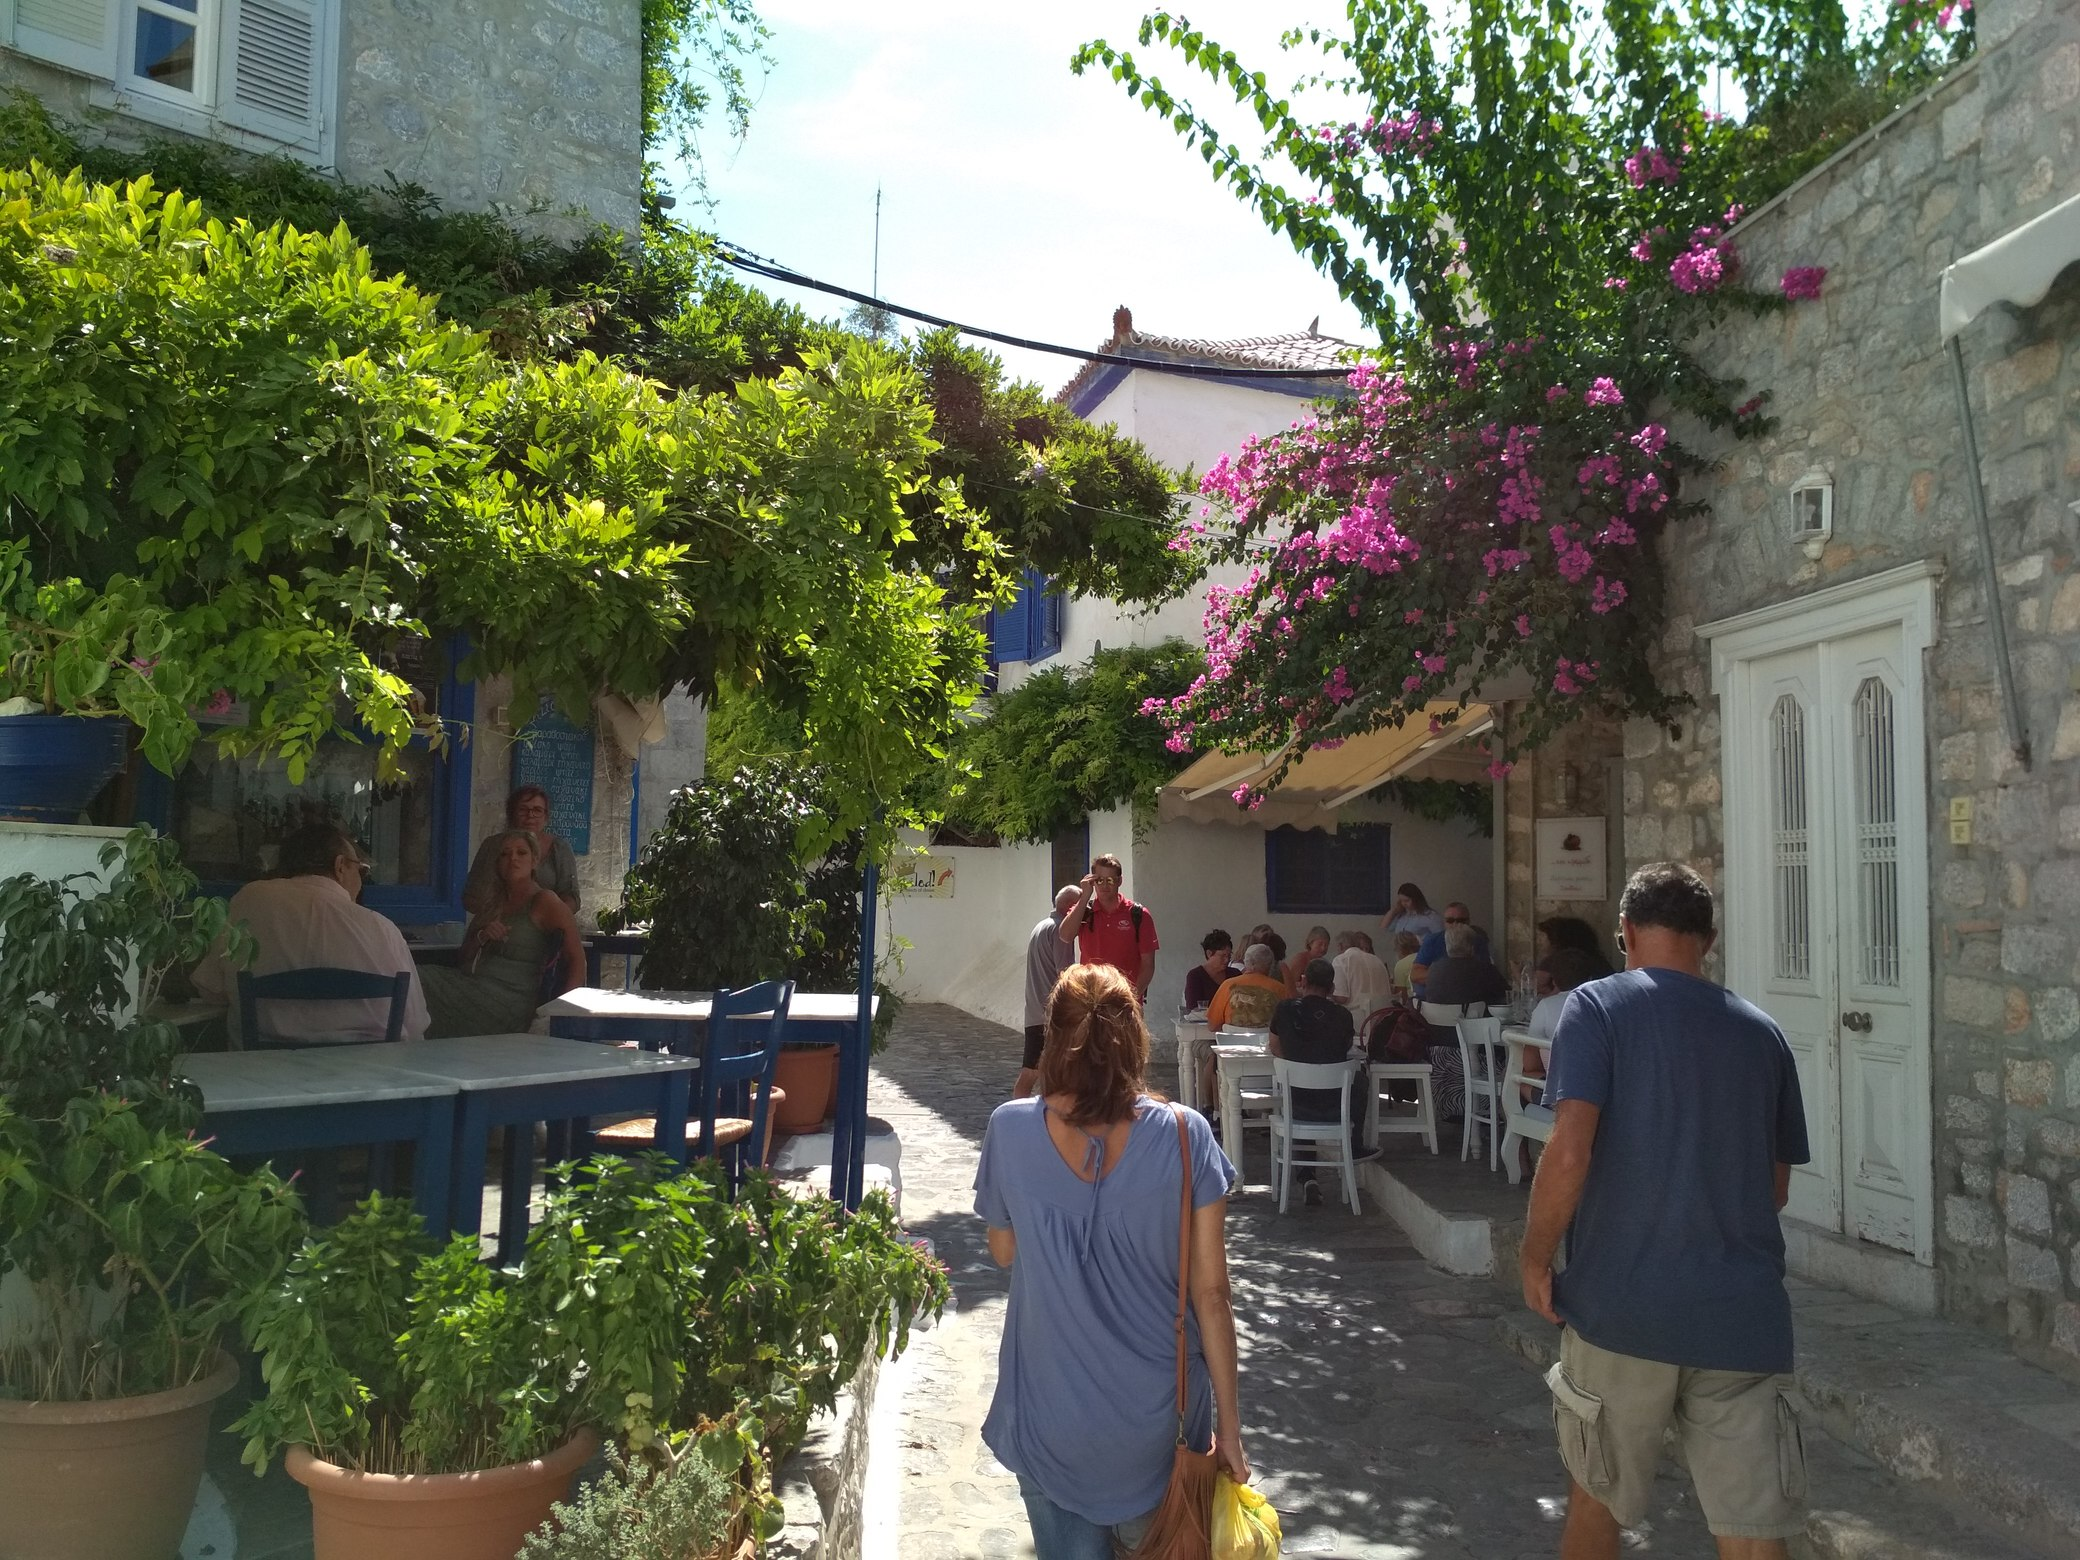
\includegraphics[width=0.32\textwidth]{media/hydra_city}
	\par\textit{Beautiful streets of Hydra}
\end{center}


%1234567890123456789012345678901234567890123456789012345678901234567890123456789
Our boat was leaving at 20:00 o'clock, therefore, we took our time to enjoy 
the sunset from the top of cafeteria named \textbf{NAME HERE} while having 
cocktails and discussing past moments and pleasant memories from our masters. 
At some point, we had to go back and embark on the ship. 
That was the moment when Dorine said with a complaining tone in her voice 
``Why are we going back to Athens, let's stay here instead...''. 
Oh my...this attractiveness and charm of the Greek islands it is imaginable.


%----------------------------------------------------------------------------------------
\NewsItem{What have I learned?}

%1234567890123456789012345678901234567890123456789012345678901234567890123456789
Proper preparation before every adventure is crucial, especially for places that I 
have never visited before. 
Getting temperature and wind's [measurements] is important to adjusts your clothing, 
food and water supplies, and exploiting transportation options is important, but, 
having great, bad-ass, and crazy companions is even more important. 
When things are not proceed as I planned that makes, on the same time, a new funny 
story to discuss and laugh about it with friends.     
By the end of the day, never forget to enjoy the sunset since it is one the worlds 
wonders, it is magical, and free! 
Also, I carry with me wireless speakers to enjoy music at every moment. 
In my case, I use the water-proof wireless speakers EU roll 2 (a birthday present 
from my dear friends Daniela and Antonis) during hiking or laying on beach. 


%----------------------------------------------------------------------------------------
\NewsItem{Acknowledgments}

%1234567890123456789012345678901234567890123456789012345678901234567890123456789
Greek islands are magical places with many beauties blooming during the whole year, 
a place that one could easily describe as paradise. 
Staying here for almost three years it offered me so much in terms of knowledge, 
life experience, traveling, and adventure. 
I would like to deeply thank all my friends who contributed in making my journey 
and accommodation an unforgettable memory and carved unique moments of joy 
and happiness that I will always carry with me. 
Cheers guys, let's do it again soon!!!


\end{multicols}

% Discuss about Hydra and how Dorine was saying...can we not go back to Athens and stay here?
\begin{center}
	\includegraphics[width=1\textwidth]{media/my_friends}
	\par\textit{Thank you all for the great company and the unforgettable moments (could not fit any more people in the frame, so please forgive me if I left someone outside)}
\end{center}



\end{document} 
